\section{~数值方法} \label{chapt:num}
\newcounters

% 本章正文正按 \input 文件逐节替换为中文。
Cartesian 坐标（\ref{eq:bal_plane}）或球坐标（\ref{eq:bal_sphere}）中的波作用量方程，是波浪模式的基本方程。不过，模式中使用的是这些方程的修正形式，其中：(a) 方程在可变波数网格上求解（见下文）；(b) 在选定数值格式中使用方程的修正形式，以正确描述离散方程的色散（见 \para\ref{sub:xy_prop}）；(c) 考虑岛屿等子网格障碍物（见 \para\ref{sub:xy_prop}）。


\vssub
\subsection{~谱离散} \label{sec:basic_num}
\vsssub


如果直接求解式 (\ref{eq:bal_plane}) 或式 (\ref{eq:bal_sphere})，在浅水中会出现有效谱分辨率降低 \citep[见][]{tol:GAOS98b}。如果方程在可变波数网格上求解，则可避免这种分辨率损失；该网格隐式包含了浅化导致的运动学波数变化。这样的波数网格对应于相对频率中空间和时间不变的网格 \citep{tol:GAOS98b}。相应的局地波数网格可由不变频率网格和色散关系 (\ref{eq:disp}) 直接计算，因此成为局地水深 $d$ 的函数。为便于经济地计算 $S_{nl}$，并让涌浪频率得到良好分离，采用频率间隔指数增长的频率离散，使变化的频率分辨率与局地频率成正比：

%----------------------------%
% Exponential frequency grid %
%----------------------------%
% eq:sigma_grid

\begin{equation}
\sigma_{m+1} = X_\sigma \, \sigma_m \: , \label{eq:sigma_grid}
\end{equation}

\noindent
其中 $m$ 是 $k$ 空间中的离散网格计数器。$X_\sigma$ 由用户在程序输入文件中定义。传统上，在第三代模式的大多数应用中使用 $X_\sigma \simeq 1.1$。

这里只针对 Cartesian 方程 (\ref{eq:bal_plane}) 讨论空间变化网格的影响。改写到球面网格是直接的。用 $\kappa$ 表示可变波数网格时，平衡方程变为

%------------------------------%
% general equations kappa-grid %
%------------------------------%
% eq:bal_f_grid
% eq:sigma_dot

\begin{equation}
\frac{\p}{\p t} \frac{N}{c_g} +  
\frac{\p}{\p x} \frac{\dot{x} N}{c_g} + 
\frac{\p}{\p y} \frac{\dot{y} N}{c_g} + 
\frac{\p}{\p \kappa} \frac{\dot{\kappa} N}{c_g} + 
\frac{\p}{\p \theta} \frac{\dot{\theta} N}{c_g}  =
\frac{S}{\sigma c_g} \: , \label{eq:bal_f_grid} \end{equation} \begin{equation}
\dot{\kappa} \:\frac{\p k}{\p \kappa} =
     c_g^{-1} \frac{\p \sigma}{\p d} \left (
    \frac{\p d}{\p t} + {\bf U} \cdot \nabla_x d \: \right ) -
    {\bf k} \cdot \frac{\p {\bf U}}{\p s}
\: . \label{eq:sigma_dot}
\end{equation}

\noindent

\vssub
\subsection{~波作用量方程的分裂} \label{sec:basic_num}
\vsssub

在 \ws\ 中，式 (\ref{eq:bal_f_grid}) 使用分步法求解。第一步处理水深的时间变化以及相应的波数网格变化。如 \cite{tol:GAOS98b} 所讨论的，这一步可较低频率地调用。通过把水位（时间）变化的影响分离出去，网格变为不变网格，并且在剩余分步中水深可视为准定常。其他分步处理空间传播、谱内传播和源项。从 5.10 版开始，源项 $S$ 进一步分裂为非冰源项 $S_{no~ice}$ 和冰源项 $S_{ice}$。对于单个模式网格，{\code W3WAVE} 例程执行如下积分序列：
\begin{itemize}
 \item[1.] 更新水位
 \item[2.] 谱内部分 1：在 $\Delta t_g/2$ 上积分 $\frac{\p}{\p t} \frac{N}{c_g} + \frac{\p}{\p \kappa} \frac{\dot{\kappa} N}{c_g} + \frac{\p}{\p \theta} \frac{\dot{\theta} N}{c_g}  =0 $
 \item[3.] 空间传播：在 $\Delta t_g$ 上积分 $\frac{\p}{\p t} \frac{N}{c_g} +  
\frac{\p}{\p x} \frac{\dot{x} N}{c_g} + 
\frac{\p}{\p y} \frac{\dot{y} N}{c_g}  = 0$
 \item[4.] 谱内部分 2：在 $\Delta t_g/2$ 上积分 $\frac{\p}{\p t} \frac{N}{c_g} + \frac{\p}{\p \kappa} \frac{\dot{\kappa} N}{c_g} + \frac{\p}{\p \theta} \frac{\dot{\theta} N}{c_g}  =0 $
 \item[5.] 源项积分：在 $\Delta t_g$ 上积分 $\frac{\p}{\p t} \frac{N}{c_g}   = \frac{S_{no~ice}}{\sigma c_g}$
 \item[6.] 冰源项积分：在 $\Delta t_g$ 上积分 $\frac{\p}{\p t} \frac{N}{c_g}   = \frac{S_{ice}}{\sigma c_g}$
\end{itemize}
在 $\Delta t_g \rightarrow 0$ 的极限下，这 6 个步骤的连续执行等价于在全局时间步长 $\Delta t_g$ 上积分式 (\ref{eq:bal_f_grid})。

这种多步骤分裂允许同时进行高效的向量化和并行化。时间分裂还允许在模式不同分步中使用独立的部分时间步长或动态调整的时间步长。\ws\ 区分 4 种不同的时间步长。\label{dt_list}

\begin{list}{xx}{\itemsep 0mm \parsep 0mm \rightmargin 5mm}

\item[1)] “全局”时间步长 $\Delta t_g$ 是所有分裂子积分的公共步长。在这个意义上，它是能够得到物理上有意义解的最小时间步长，因为方程中的所有项都已积分。因此，它可作为评估模式输出或与其他模式耦合的时间步长；在多网格系统中，它也是网格间通信所采用的时间步长。对于强迫模式（而非耦合模式），输入风和流在该全局步长上插值。该时间步长由用户在 {\code ww3\_grid} 输入文件中给出，但模式内部可将其缩小，以满足所要求的输入或输出时刻。

\item[2)] 第二种时间步长是空间传播时间步长。它不用于基于三角形的网格；对此类网格，在显式格式中，平流步长会在内部对每个谱分量调整。对于其他网格类型，用户在无流且网格不运动的假设下，为最低模式频率提供一个参考最大传播时间步长 $\Delta t_{p,r}$。对计数器为 $m$ 的频率，最大时间步长 $\Delta t_{p,m}$ 在模式内部计算为

%-------------------------%
% Time stepping equations %
%-------------------------%
% eq:dtpl

\begin{equation}
\Delta t_{p,m} = \frac{{\dot{x}}_{p,r}}{{\dot{x}}_{p,m}} \Delta t_{p,r}
\: , \label{eq:dtpl} \end{equation}

\noindent
其中 $\dot{x}_{p,r}$ 为无流且网格不运动时最长波的最大平流速度，$\dot{x}_{p,m}$ 为频率 $m$ 的实际最大平流速度（包括流）。如果传播时间步长小于全局时间步长，则传播效应用多个连续的较小时间步长计算。这通常意味着最低频率会使用多个部分时间步，而最高频率在 $\Delta t_g$ 间隔内只需一次计算即可传播。后者可显著提高模式效率，特别是在使用高阶精度传播格式时。注意，$\Delta t_{p,m}$ 可定义为大于 $\Delta t_g$，这对有（强）流情形下的模式经济性可能有影响。

\item[3)] 第三种时间步长是谱内传播时间步长。对于大尺度和深水网格，该时间步长通常可取为全局时间步长 $\Delta t_g$。对于浅水网格，在格式稳定性约束内，较小的谱内传播时间步长可允许更强的折射效应。注意，为提高数值精度，空间传播和谱内传播的调用顺序会交替。如果长周期涌浪发生强折射，这可能导致平均波浪参数出现明显起伏。可通过把该时间步长设为 $\Delta t_g$ 的偶数整数分数来避免这种情况。

\item[4)] 最后一种时间步长是源项积分时间步长，它会针对每个独立网格点和每个全局时间步长 $\Delta t_g$ 动态调整（见 \para~\ref{sub:source}）。这使快速变化的风和波浪条件计算更准确，同时也使缓慢变化条件下的积分更经济。为限制计算时间，用户需定义最小时间步长。

\end{list}

\vspace{\baselineskip} \noindent 

以下各节讨论分步法中的各个独立步骤，以及与之相关的若干问题。主要内容包括：\para\ref{sub:num_depth} 讨论水深时间变化的处理；\para\ref{sub:xy_prop} 讨论空间传播；\para\ref{sub:spec} 讨论谱内传播；第 \ref{sub:source} 和 \ref{sub:icesource} 节讨论非冰和冰源项的数值积分。其他小节讨论附加数值方法和技术，包括风和流的处理（\para\ref{sub:num_w_c}）、潮汐（\para\ref{sub:num_tide}）、时空极值计算（\para\ref{sub:space_time_ext}）、海冰处理（\para\ref{sub:num_ice}）、谱分区以及波系在空间和时间中的相应追踪（第 \ref{sub:num_part}、\ref{sub:num_track} 节），以及嵌套（\para\ref{sub:num_nest}）。

\vssub
\subsection{~水深随时间变化} \label{sub:num_depth}
\vssub

水深的时间变化会导致局地波数网格改变。由于波数谱相对于水深时间变化是不变的，这对应于把谱从旧网格简单插值到新网格，而不改变谱形。如上文所述，新网格直接由全局不变的频率网格、新水深 $d$ 和色散关系式 (\ref{eq:disp}) 得到。更新水位的时间步长通常由水位变化的物理时间尺度决定，而不是由数值考虑决定 \citep{tol:GAOS98b}。

插值到新波数网格时使用一种简单的守恒插值方法。在该插值中，先将旧谱乘以谱箱宽度，转换为离散作用量密度。随后按常规线性插值方式，把该离散作用量重新分配到新网格上。新的离散作用量再除以（新的）谱箱宽度，转换回谱。由于旧网格通常不会完全覆盖新网格，该转换需要在高频和低频处对原始谱作参数化延拓。旧谱中位于低波数、且不被新网格解析的能量/作用量会被直接移除。新网格中位于低波数、且不被旧网格解析的部分假定能量/作用量为零。在新网格的高波数处，必要时采用通常的参数化谱尾。后一种修正较少发生，因为最高波数通常对应深水。

在实际应用中，网格修正通常只与少部分网格点有关。为避免不必要计算，仅当离散谱中最小相对水深 $kd$ 小于 4 时才变换网格。此外，仅当空间网格点未被冰覆盖，且最大波数变化至少为 $0.05 \Delta k$ 时，才对谱进行插值。

\vssub
\subsection{~空间传播} \label{sub:xy_prop}
\vssub
\subsubsection{~一般概念}
\vsssub

\ws\ 中的空间传播由式 (\ref{eq:bal_f_grid}) 的前几项描述。对于球坐标 [式 (\ref{eq:bal_sphere})]，相应的空间传播步骤为

%----------------------------%
% Step : Spatial propagation %
%----------------------------%
% eq:step_xy_prop

\begin{equation}
\frac{\p \cN}{\p t} + \frac{\p}{\p \phi} \, \dot{\phi} \cN +
\frac{\p}{\p \lambda} \, \dot{\lambda} \cN = 0
\: , \label{eq:step_xy_prop} 
\end{equation}

\noindent 
其中被传播的量 $\cN$ 定义为 $\cN \equiv N \, c_g^{-1} \, \cos\phi$。对于 Cartesian 网格，可得到类似方程，其中 $\cN \equiv N \, c_g^{-1}$。本节仅给出更复杂的球面网格方程。转换到 Cartesian 网格通常是一种简化，而且是直接的。

式~(\ref{eq:step_xy_prop}) 在形式上与常规深水传播方程相同，但同时包含有限水深和流的影响。在陆海边界处，假定向陆地传播的波作用量被吸收且不反射，离岸传播的波在岸线处假定无能量。对于规定边界条件的所谓“活动边界点”，也采用类似方法。传播到这些点的作用量被吸收，而边界点处的作用量用于估计进入模式的分量的作用量通量。

空间网格可使用两种不同坐标系统：一种是“平面” Cartesian 坐标系，通常用于小尺度和理想化测试应用；另一种是球面（纬度-经度）系统，用于大多数真实应用。在模式 3.14 版中，坐标系统通过 {\code XYG} 或 {\code LLG} 开关在编译时选择。在较新的模式版本中，网格类型已成为在 {\file ww3\_grid} 中定义并存储于 {\file mod\_def.ww3} 文件中的变量。

球面网格可选择简单闭合，使其在经度方向周期化，例如能量可从网格最大经度向东传播到网格最小经度。该闭合之所以称为“简单”，是因为跨过这条“接缝”时纬度索引不变。也允许“非简单”闭合类型，它与三极网格有关。三极网格是一种不规则网格，因此该闭合将在 (\ref{sub:num_space_curv}) 中进一步讨论。
 
直到模式 3.14 版，\ws\ 只考虑规则离散网格，其中两个主网格轴 ($x,y$) 使用常数增量 $\Delta x$ 和 $\Delta y$ 离散。在模式 \WWver\ 中，加入了包括曲线网格和非结构网格在内的附加选项。以下小节将先讨论这些网格方法，然后再处理额外的传播问题，包括 Garden Sprinkler Effect（\ref{sub:num_GSE}）、连续移动网格（\ref{sub:num_move}）、未解析岛屿（\ref{sub:num_obst}）和旋转网格（\ref{sub:num_space_rotagrid}）。

\vssub
\subsubsection{~传统规则网格} \label{sub:num_space_trad}

\noindent
传统规则网格的传播格式在编译时通过开关选择。\ws\ 中提供了若干格式。下面按复杂程度递增的顺序介绍这些格式。

\addcontentsline{toc}{subsubsection}{\strut \hspace{24mm} 一阶格式}

\vspace{\baselineskip} 
\vspace{\baselineskip} 
\noindent {\bf 一阶格式}

\opthead{PR1}{\ws}{H. L. Tolman}

\noindent
模式中包含了一个简单而低成本的一阶迎风格式，主要用于 \ws\ 开发过程中的测试。为保证作用量的数值守恒，采用通量或控制体积形式。在 $\phi$ 空间中，计数器为 $i$ 和 $i-1$ 的网格点之间的通量 $(\cF_{i,-})$ 计算为

% ------ First order scheme ------- %
% eq:1up_xy_1        Basic flux
% eq:1up_xy_2        Boundary velocity
% eq:1up_xy_3        Upstream value

\begin{equation}
\cF_{i,-} = \left [ \: \dot{\phi}_b \: \cN_u \: \right ]^n_{j,l,m}
\: , \label{eq:1up_xy_1} \end{equation} \begin{equation}
\dot{\phi}_b = 0.5 \: \left ( \dot{\phi}_{i-1} + \dot{\phi}_i 
\: \right )_{j,l,m} \: , \label{eq:1up_xy_2}
\end{equation} \begin{equation}
\cN_u = \left \{ \begin{array}{ccc}
\cN_{i-1} & \mbox{for} & \dot{\phi}_b \geq 0 \\
\cN_i     & \mbox{for} & \dot{\phi}_b   <  0
\end{array} \right . \: , \label{eq:1up_xy_3}
\end{equation}

\noindent
其中 $j$、$l$ 和 $m$ 分别为 $\lambda$、$\theta$ 和 $k$ 空间中的离散网格计数器，$n$ 为离散时间步计数器。$\dot{\phi}_b$ 表示点 $i$ 与 $i-1$ 之间“单元边界”处的传播速度，下标 $u$ 表示“上游”网格点。在陆海边界处，$\dot{\phi}_b$ 由海点处的 $\dot{\phi}$ 代替。点 $i$ 与 $i+1$ 之间的通量 $(\cF_{i,+})$ 通过把 $i-1$ 替换为 $i$、把 $i$ 替换为 $i+1$ 得到。$\lambda$ 空间中的通量以类似方式计算，只需改变相应的网格计数器和增量。时间 $n+1$ 的“作用量密度” $(\cN^{n+1})$ 估计为

% eq:1up_xy_tot

\begin{equation}
\cN_{i,j,l,m}^{n+1} = \cN_{i,j,l,m}^n
  + \frac{\Delta t}{\Delta \phi   } \left [ \cF_{i,-} - \cF_{i,+} \right ]
  + \frac{\Delta t}{\Delta \lambda} \left [ \cF_{j,-} - \cF_{j,+} \right ]
\: , \label{eq:1up_xy_tot}
\end{equation}

\noindent
其中 $\Delta t$ 为传播时间步长，$\Delta \phi$ 和 $\Delta \lambda$ 分别为纬度和经度增量。在陆地上取 $\cN=0$ 时，式 (\ref{eq:1up_xy_1}) 至 (\ref{eq:1up_xy_3})，并且仅在海点上应用式 (\ref{eq:1up_xy_tot})，会自动调用所需边界条件。

注意，式~(\ref{eq:1up_xy_tot}) 表示该格式的二维实现，因此需要在式~(\ref{eq:dtpl}) 中使用实际平流矢量的范数。还需注意，这意味着完整方程的 CFL 判据通常比把 $\lambda$ 和 $\phi$ 传播分开处理的格式更严格；下文讨论的三阶格式即采用后者。对于两个方向网格间距相等的网格，一阶格式的最大时间步长比三阶格式小 $1/\sqrt{2}$ 倍。

\addcontentsline{toc}{subsubsection}{\strut \hspace{24mm} 二阶格式
  (UNO)}

\vspace{\baselineskip} 
\vspace{\baselineskip} 
\noindent {\bf 二阶格式 (UNO)}

\opthead{UNO}{MetOffice}{J.-G. Li}

\noindent
上游非振荡二阶（UNO）平流格式 \citep{art:Li08} 是 MINMOD 格式 \citep{art:Roe86} 的扩展。在 UNO 格式中，单元 \emph{i}-1 与单元 \emph{i} 之间单元面中通量点处的插值波作用量值为
\begin{equation}
N_{i-}^{*}=N_{c}+sign\left(N_{d}-N_{c}\right)\frac{\left(1-C\right)}{2}\min\left(|N_{u}-N_{c}|,|N_{c}-N_{d}|\right) \:\:\: ,
\label{eq:UNO2regular}
\end{equation}

\noindent
其中 \emph{i}- 为单元面索引；$C=\left|\dot{\phi_{b}}\right|\Delta t/\Delta\phi$ 为绝对 CFL 数；下标 \emph{u}、\emph{c} 和 \emph{d} 分别表示相对于给定 \emph{i}- 单元面速度 $\dot{\phi}_{b}$ 的\emph{上游、中心}和\emph{下游}单元。若 $\dot{\phi}_{b}>0$，则对单元 \emph{i}-1 与单元 \emph{i} 之间的单元面，有 \emph{u} = \emph{i}-2、\emph{c}=\emph{i}-1、\emph{d}=\emph{i}。若 $\dot{\phi}_{b}\leq0$，则 \emph{u}=\emph{i}+1、\emph{c}=\emph{i}、\emph{d}=\emph{i}-1。UNO 格式的细节见 \cite{art:Li08}，其中还给出了标准数值测试，证明只要 CFL 数小于 1.0，Cartesian 多单元网格上的 UNO 格式就是非振荡、守恒、保持形状的，并且比其经典对应格式更快。

通量和单元值更新采用与一阶上游格式相同的形式，即

\begin{equation}
\mathcal{F}_{i-}=\dot{\phi_{b}N_{i-}^{*}};\;\;\; N_{i}^{n+1}=N_{i}^{n}+\frac{\Delta t}{\Delta\phi}\left(\mathcal{F}_{i-}-\mathcal{F}_{i+}\right) \:\:\: ,
\end{equation}
 
\noindent
其中 $\mathcal{F}_{i+}$ 是单元 \emph{i} 与单元 \emph{i}+1 之间单元面的通量。它可用类似于 (\ref{eq:UNO2regular}) 的中通量值估计，只需把 \emph{i} 替换为 \emph{i}+1。为把 UNO 格式扩展到多维，采用可减小时间分裂误差的平流-守恒混合算子 \citep{art:LLM96}。


\addcontentsline{toc}{subsubsection}{\strut \hspace{24mm} 三阶格式 (UQ)}

\vspace{\baselineskip}
\vspace{\baselineskip} 
\noindent {\bf 三阶格式 (UQ)}

\opthead{UQ}{\ws}{H. L. Tolman}

\noindent 
\ws\ 中可用的三阶精度格式为 \qck\ 格式 \citep{art:Leo79,art:DM82}，并结合 \ult{} \tvd{}（总变差递减）限制器 \citep{art:Leo91}。这是 \ws\ 的默认传播格式。该格式在空间和时间上均为三阶精度，选择它是基于水质模式中高阶有限差分格式的大量相互比较 \citep[见][]{PhD:Cah,pro:FC93,tol:OMB95}。该格式分别应用于经向和纬向传播，并交替改变首先处理的方向。

在 \qck\ 格式中，$\phi$ 空间中计数器为 $i$ 和 $i-1$ 的网格点之间的通量 $(\cF_{i,-})$ 计算为\footnote{~计数器为 $i+1$ 和 $i$ 的网格点之间的通量 $(\cF_{i,+})$ 仍通过替换相应索引得到。}

% ------ QUICKEST scheme ---------- %
% eq:quick_1         Basic flux
% eq:quick_2         Boundary value
% eq:quick_3         Divergence
% eq:quick_4         CFL number

\begin{equation}
\cF_{i,-} = \left [ \dot{\phi}_b \: \cN_b \: \right ]^n_{j,l,m} \: , \label{eq:quick_1}
\end{equation} \begin{equation}
\dot{\phi}_b = 0.5 \: \left ( \dot{\phi}_{i-1} + \dot{\phi}_i 
\: \right ) \: , \label{eq:quick_1a}
\end{equation}  \begin{equation}
\cN_b = \frac{1}{2} \left [ \rule[0mm]{0mm}{\baselineskip} \: 
(1+C)\cN_{i-1} + (1-C)\cN_i \: \right ] - \:
\left ( \frac{1-C^2}{6} \right ) \: {\cal CU} \: \Delta\phi^2, \label{eq:quick_2} \end{equation} \begin{equation}
{\cal CU} =  \left \{ \begin{array}{ccc}
(\: \cN_{i-2} - 2\cN_{i-1} + \cN_{i} \:)\: \: \Delta \phi^{-2}
               & \mbox{for} & \dot{\phi}_b \geq 0 \\
(\: \cN_{i-1} - 2\cN_{i} + \cN_{i+1} \:)\: \Delta \phi^{-2}
               & \mbox{for} & \dot{\phi}_b   <  0
\end{array} \right . \: , \label{eq:quick_3}
\end{equation} \begin{equation}
C = \frac{\dot{\phi}_b \: \Delta t}{\Delta \phi} 
\: , \label{eq:quick_4} \end{equation}

\noindent
其中 $\cal CU$ 是作用量密度分布的（上游）曲率，$C$ 是带符号的 \cfl\ 数，用来标识传播方向。与一阶格式类似，当 $|C| \leq 1$ 时该格式给出稳定解。为保证该格式不产生非物理极值，它与 \ult\ 限制器结合使用。该限制器使用中心、上游和下游作用量密度（下标分别为 $c$、$u$ 和 $d$），定义为

% ------ ULTIMATE limiter --------- %
% eq:ult_1           Cell definition
% eq:ult_2           Nondimensional action
% eq:ult_3           Monotonic limiter
% eq:ult_4           Non-monotonic action

\begin{equation} \begin{array}{ccccc}
\cN_c = \cN_{i-1} \: , \: & \cN_u = \cN_{ i-2 } \: , \: &
                            \cN_d = \cN_{i} &
                            \mbox{for} & \dot{\phi}_b \geq 0 \\
\cN_c = \cN_{ i } \: , \: & \cN_u = \cN_{i+1} \: , \: &
                            \cN_d = \cN_{i-1} &
                            \mbox{for} & \dot{\phi}_b   <  0
\end{array} \: . \label{eq:ult_1} \end{equation}

\noindent
为评估初始状态与解是否表现出相似的单调或非单调行为，定义归一化作用量 $\tilde\cN$：

\begin{equation}
\tilde\cN = \frac{\cN-\cN_u}{\cN_d - \cN_u} 
\: . \label{eq:ult_2} \end{equation}

\noindent
若初始状态是单调的（即 $0 \leq \tilde\cN_c \leq 1$），则单元边界处的（归一化）作用量 $\cN_b$ 被限制为

\begin{equation}
\tilde\cN_c \leq \tilde\cN_b \leq 1 , \:\:\:
\tilde\cN_b \leq \tilde\cN_c \: C^{-1}  . 
\label{eq:ult_3} \end{equation}
\noindent 否则 \begin{equation}
\tilde\cN_b = \tilde\cN_c 
\: . \label{eq:ult_4} \end{equation}

\noindent
如果与单元边界相邻的两个网格点之一位于陆地上，或表示活动边界点，则需要使用另一种格式。在这些情况下，式~(\ref{eq:1up_xy_2}) 和 (\ref{eq:quick_2}) 由下式代替：

% eq:1_vel           Boundary velocity
% eq:1_bval          Boundary value

\begin{equation}
\dot{\phi}_b = \dot{\phi}_s \: ,
\label{eq:1_vel} \end{equation} \begin{equation}
\cN_b = \cN_u \: ,
\label{eq:1_bval} \end{equation}

\noindent
其中后缀 $s$ 表示海点的（平均）值。该边界条件表示一个简单的一阶迎风格式，不需要式 (\ref{eq:ult_1}) 至 (\ref{eq:ult_4}) 的限制器。

最终传播格式类似于式~(\ref{eq:1up_xy_tot})，为

% eq:uq_xy_tot

\begin{equation}
\cN_{i,j,l,m}^{n+1} = \cN_{i,j,l,m}^n +
\frac{\Delta t}{\Delta \phi} \left [ \cF_{i,-} - \cF_{i,+} \right ]
\: . \label{eq:uq_xy_tot} \end{equation}

\noindent
$\lambda$ 空间中的传播格式只需在上述方程中轮换索引和增量即可得到。\footnote{~\cite{tol:OMB02c} 第 31 页所述的“软”边界处理已不再可用，因为它与模式 3.14 版引入的高级嵌套技术不兼容。}

注意，\uq\ 格式实现为交替的一维格式，因此需要在式~(\ref{eq:dtpl}) 中使用分量平流速度的最大值。为保持一致，对于给定分量，$\lambda$ 和 $\phi$ 传播始终使用相同时间步长。

\vssub
\subsubsection{~曲线网格} \label{sub:num_space_curv}
\conthead{\ws (NRL Stennis)}{W. E. Rogers, T. J. Campbell}

\noindent 
作为传统“规则”网格的扩展，\ws\ 可在“不规则”网格上进行计算。这使模式可运行于替代网格投影（例如 Lambert 正形圆锥投影）、旋转网格，或近岸分辨率更高的贴岸线网格；不过，条件稳定格式对时间步长的限制仍然适用。不规则网格使用的传播格式与规则网格相同（\para\ref{sub:num_space_trad}）。

其实现由 \cite{rep:RC09} 详细描述，这里概述如下：使用 Jacobian 在整个区域内将正常的曲线空间与拉直空间相互转换。该转换只在传播例程内部进行，而不是在拉直空间中积分整个模式。每次调用传播子程序时（即每个时间步和每个谱分量），采用一个简单的三步过程：第一，用 Jacobian 把因变量（波作用量密度）转换到拉直空间；第二，通过对两个网格轴分别调用子程序来传播波作用量密度；第三，把波作用量密度转换回正常的曲线空间。实际通量计算相对于原来的规则网格形式没有显著改变。无论网格类型（规则或不规则）如何，都采用同一过程；对于规则网格，Jacobian 为 1。

关于用户接口：在 {\file ww3\_grid.inp} 中，用字符串表示网格类型。当该网格字符串为 `{\code RECT}' 时，模式处理规则网格输入。当该网格字符串为 `{\code CURV}' 时，模式处理不规则网格输入。[注意，在 \ws\ 4.00 版中，坐标系统（即度或米）和闭合类型（例如全球/环绕网格）也在 {\file ww3\_grid.inp} 中指定；开关 {\code LLG} 和 {\code XYG} 已废弃。]

从 \ws\ 第 5 版起，增加了在一种特殊曲线网格即“三极网格”上使用一阶传播格式运行的能力。在北半球，该网格类型使用两个极点而不是一个，并且两个极点都位于陆地上，以避免网格距奇异性。这类网格有时用于海洋模式，例如 \citep{art:Murr96} 和 \citep{art:Metz14}。不需要特殊开关，网格像其他不规则网格一样读入，但用户必须在 {\file ww3\_grid.inp} 中指定闭合类型 ({\code CSTRG}) 为 {\code TRPL}。具体细节见 \para\ref{sub:ww3grid} 中 {\file ww3\_grid.inp} 的文档。传播和梯度计算已修改，以处理新的闭合方法。{\code TRPL} 闭合类型仅与一阶 {\code PR1} 传播格式兼容。三极网格的一个吸引人特性是，它允许用户运行一个一直延伸到北极的单一网格。不过，虽然三个极点都位于陆地上，最靠近它们的海点处仍存在经线汇聚，这意味着以真实距离表示的网格距（决定最大传播时间步长）仍高度变化。通过使用多网格能力，可以获得更高效的网格距（即真实距离上的网格距变化较小）。虽然该格式处理了极点处网格距的奇异性，但并未处理与波向定义相关的奇异性。

\vssub
\subsubsection{~三角形非结构网格} \label{sub:num_space_tri}
\conthead{WWM-II}{A. Roland, F. Ardhuin, M. Dutour-Sikiri\'c, A. Abdolali}

\noindent
在 \ws\ 中，可以选择基于三角形的非结构网格，并使用基于轮廓残差分配（CRD）的数值格式 \citep{art:ricchiuto2005} 来离散空间导数。这些格式已在 \citep{rep:Roland2008} 中应用到波作用量平衡方程，并在 Wind Wave Model-II (WWM-II) 和 WW-III 中实现。对于时间积分方法，非结构网格可使用显式和隐式格式。如果选择显式求解器，则使用 WW3 原始分步法，其中地理空间中二维双曲部分的解在非结构网格上用上述方法求解。在这种情况下，谱部分和源项的积分方式与 WW3 结构网格版本类似。时间步长定义也与结构网格部分相同，只是非结构部分的子迭代次数会根据区域内最大 CFL 数自动估计。若选择隐式方法，则根据 \citep{rep:Roland2008}，基于 CRD-N 格式组装线性方程组。谱传播部分用简单的隐式一阶迎风格式求解，源项则以与 WW3 动态格式相同的方式写入矩阵，即在式 3.61 中取 $\epsilon = 1$，并按简单 Patankar 规则组装方程组。新实现的完整说明见 \cite{rolandetal2019t}。可以通过解析推导和数值实验表明，当 CFL \textless 1 时，显式和隐式方法给出相似结果。这也已在实际应用中得到展示，例如 \citep{rep:Abdolalli2018, Smith2018, rep:Abdolalli2019, AbdolaliEtAl2019OM}。不过，当 CFL \textgreater 1 时，由于源项在时间上线性化，隐式格式的瞬态解具有时间步长依赖性。隐式格式中的时间步长等于全局时间步长，谱空间或源项的其他时间步长不起作用。分步法同样由于分裂误差而具有时间步长依赖性，这在浅水中尤为显著 \citep{rep:Roland2008}。对于两类数值方法，除非给定应用的精度水平已经令人满意，否则都需要针对全局时间步长和空间分辨率进行适当的收敛性分析。随后，这些数值实现已在 WWIII 中得到评估 \citep[e.g.][]{art:Aea09,art:babanin2011,art:bertin2014,
art:bertin2015,art:dodet2013,art:ferrarin2008,art:ferrarin2013,art:janekovic2015,art:kerr2013,art:liau2011,art:Mea10,art:perrie2018,
art:perrie2013two,pro:rol2006a,pro:rol2006b,art:rol2009,art:rol2012,art:rol2014,art:sikiric2012,art:sikiric2013,art:sikiric2018,
pro:zanke2006}。


该选项通过在 {\file ww3\_grid.inp} 中把网格字符串设为 `{\code UNST}' 激活。已实现四种格式，具体选择通过 {\code UNST} namelist 完成。它们是 CRD-N 格式（一阶）、CRD-PSI 格式（优于一阶，在三角形结构网格上为二阶）、CRD-FCT 格式（二阶时空格式）和隐式 N 格式。默认格式是效率最高但扩散较强的显式 N 格式。RD 格式的一种隐式变体使用直线法和 N 格式进行空间离散，该方法由 \cite{art:Zij10} 在 SWAN 模式中实现；ECWAM 当前版本采用了类似离散，见 \cite{pro:rol2012}。

在这种方法中，节点处谱的演变（谱也在节点处求值）基于把进入与节点相关的中位对偶单元的通量收敛重新分配到节点上（见图 \ref{fig:triangles}）。对任意谱分量，平流方程式 (\ref{eq:step_xy_prop}) 在中位对偶单元上求解：进入一个单元的通量给出相应节点处波作用量的变化率。已实现的不同格式在估计该通量时采用不同离散。相关格式已在 \citep[见][综述]{rep:Roland2008} 中介绍。

需要注意的是，这些平流格式不包括 garden sprinkler effect (GSE) 修正。按照通常意义上的 GSE 修正，已发现 N 格式具有足够的数值横向扩散，可很好地补偿该效应。然而，CRD-PSI 或 CRD-FCT 等高阶格式可能根据空间分辨率产生显著 GSE 影响。

非结构网格格式的并行化可以采用与结构网格相同的 Card Deck 方法，也可以使用区域分解方法。区域分解方法基于 ParMetis \citep{rep:karypis2011metis}，后者是并行图划分算法的 C 实现。ParMetis 通过 Fortran 中的 PDLIB（Parallel Decomposition Library）接口调用；除连接 ParMetis 外，PDLIB 还按照 Fortran2002 标准提供非结构网格所需的交换例程。交换例程根据 ParMetis 提供的分解，在分解网格的不同线程之间执行所有所需通信。这样，所有区域分解部分只需一行代码即可并入主源码。要在开关文件中编译 PDLIB 选项以激活区域分解并行化，需要安装 ParMetis，并且代码需要使用 MPI 编译。PDLIB 可与所有常见 MPI 实现配合工作，例如 OpenMPI、MPICH2 等。WW3 中已实现并行算法（card deck 和区域分解）的示意图见图 \ref{DDvsCD}。对于实际应用，\cite{AbdolaliEtAl2019OM} 在 2008 年 Hurricane Ike 案例中展示了这两种方法的收敛性。

在实际中，可使用 PolyMesh 软件（由 Aron Roland 开发）由岸线多边形数据库和任意测深点列表轻松生成非结构网格。PolyMesh 连接 Triangle，并采用基于波浪传播特征的先验误差估计，以及基于重心法水深误差的深度误差估计 \citep[e.g.][]{art:WS96}。也可使用 SMS 和 OceanMesh2D 等其他网格生成工具。对三角形形状没有约束。

规则网格显式有限差分格式中 CFL 条件的等价量，是对偶单元面积除以时间步长与进入对偶单元的正波动之和的乘积。由于正通量的谱值在边界上强制给定，边界节点被排除在该 CFL 计算之外，入射能量设为零，而出射能量完全吸收。只有反射部分允许能量从边界进入区域。

岸线处的边界条件取决于波向相对于岸线取向的关系。该特殊处理通过 `{\code IOBPD}' 数组强制执行；每当网格点状态图 `{\code MAPSTA}' 改变时，该数组会更新。网格几何还用于定义局地水深和流的梯度。所有其他操作，例如把强迫插值到网格上，以及从网格插值到输出位置，均使用三角形内线性插值完成。

所有三角形几何操作都假定局地地球为平面。网格上的水深和流梯度在节点处估计，方法是在一个三角形内用线性形函数插值。

\begin{figure} \begin{center}
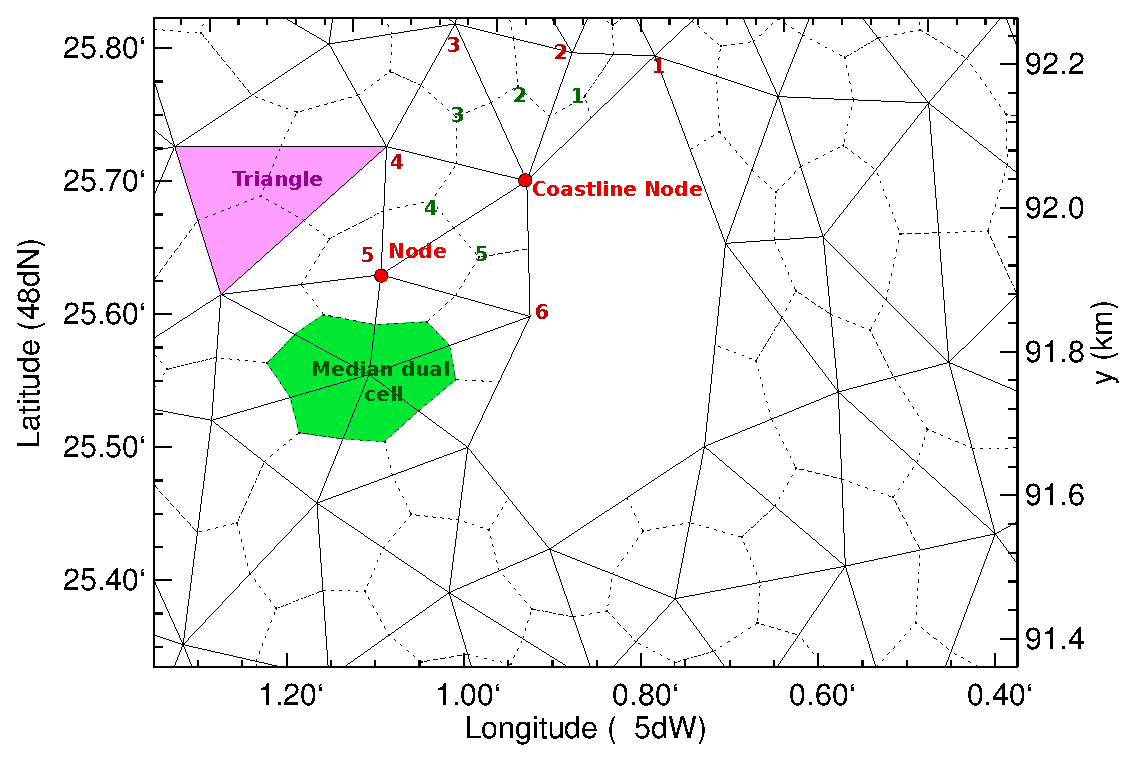
\epsfig{file=./num/grid_triangles.eps,angle=0,width=4.in}
\caption{基于三角形的网格区域示例，本例包含法国 Bannec 小岛。如果水深大于最小水深，岸线节点为活动节点。其特点是相邻节点数（所选示例中为 6）大于相邻三角形数（同一示例中为 5）。}
\label{fig:triangles} \botline
\end{center}
\end{figure}


\begin{figure} \begin{center}
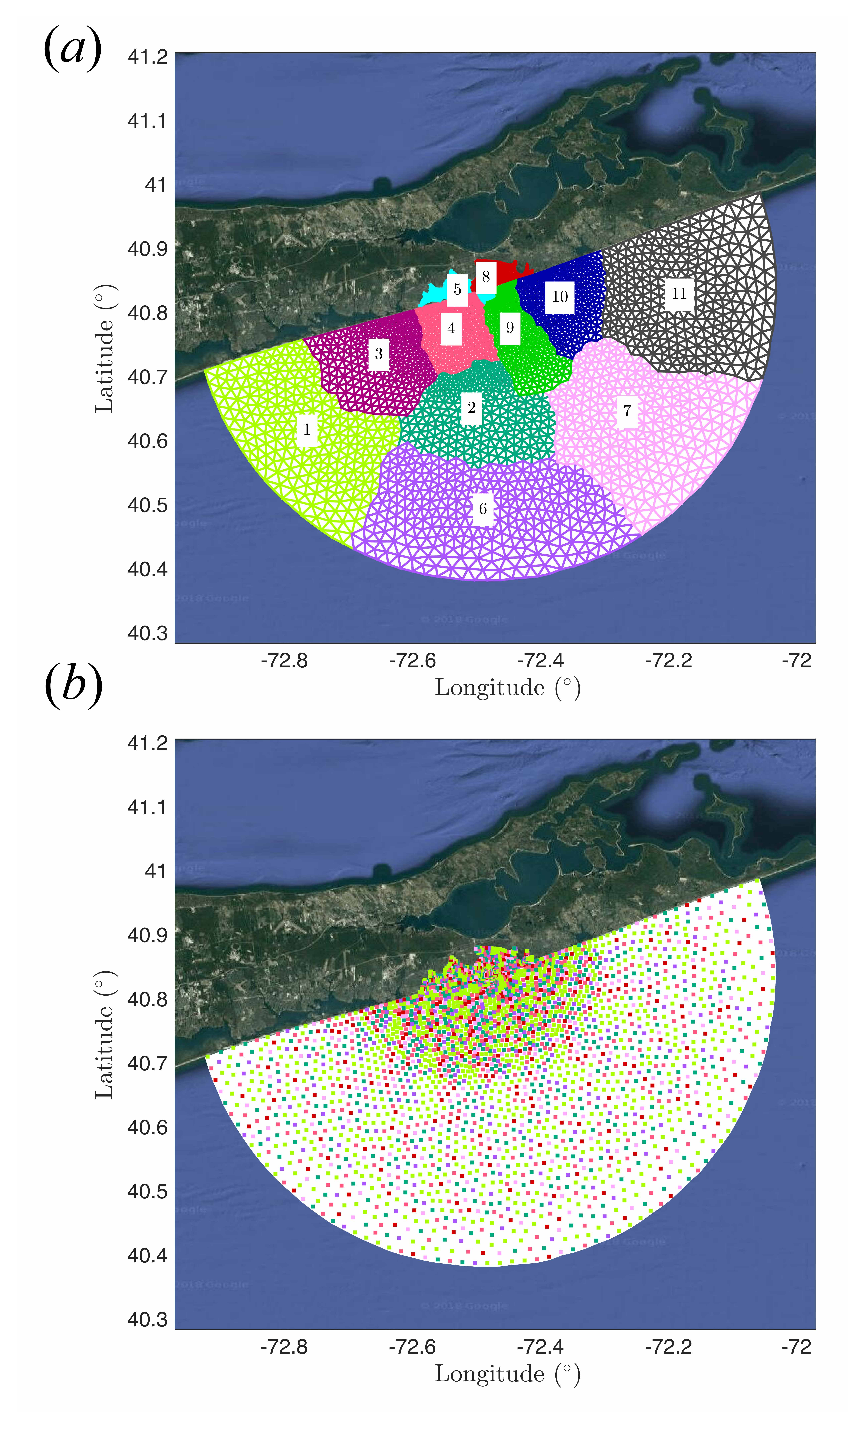
\epsfig{file=./num/DDvsCD.eps,angle=0,width=4.in}
\caption{在 11 个计算核心（以颜色表示）上，区域分解 (a) 与 Card Deck 方法 (b) 的示意差异。该网格约有 3k 个节点，针对纽约 Shinnecock Inlet 构建，取自一个 ADCIRC 示例问题。}
\label{DDvsCD} \botline
\end{center}
\end{figure}


\vssub
\subsubsection{~球面多单元（SMC）网格} \label{sub:num_space_SMC}
\opthead{SMC}{\ws (MetOffice)}{J.-G. Li}

\noindent
球面多单元（SMC）网格 \citep{art:Li11} 是 Cartesian 多单元网格 \citep{art:Li03} 向球坐标系统的扩展。它是一种非结构网格，但保留了常规经纬度网格单元，因此球坐标上的所有传播公式仍然适用，相应地所有有限差分格式也仍可使用。SMC 网格以类似于削减网格 \citep{art:RA94} 的方式放宽高纬度地区的 CFL 限制。通过转为积分方程，引入极区单元以消除微分输运方程的极点奇异性。上游非振荡二阶（UNO）平流格式 \citep{art:Li08} 已在 SMC 网格上实现，用于空间传播和谱间传播。UNO2 格式可通过 {\F PSMC} namelist 逻辑变量 {\code UNO3} 替换为三阶格式。UNO3 格式类似于 UQ 格式，但把其通量限制器替换为 UNO2 格式。波浪折射诱导旋转和大圆转向采用一种简单旋转格式 \citep{art:Li12}。对于任意时间步长，折射格式都是无条件稳定的，但最大折射诱导旋转角受到朝向局地梯度方向的最大可能折射角限制。除这一物理限制器外，{\F PSMC} namelist 中还有用户定义参数 {\code RFMAXD}，用于限制每个时间步的最大折射角。其默认值为 36.0 度。为减轻 garden sprinkler effect，使用类似 \cite{art:BH87} 的扩散项，但扩散系数简化为单一均匀参数（式~(\ref{eq:Dnn_d}) 中的 $D_{nn}$）。还可通过 {\F PSMC} namelist 逻辑变量 {\code AVERG} 使用附加的 1-2-1 加权平均格式。与常规网格相比，SMC 网格可显著减少计算时间，这得益于高纬度时间步限制的放宽以及从模式中移除陆点。为修正高纬度地区无效的标量假设，提供了一种补救方法，可将全球波浪模式扩展到整个北冰洋 \citep{art:Li16}。该 Arctic 部分可通过设置 {\F PSMC} namelist 参数 {\code Arctic=.TRUE.} 激活。

SMC 网格可用于替代规则经纬度网格，使模式区域可扩展到高纬度甚至北极，而无需缩短时间步长。除准备少量额外输入文件（包括单元数组和面数组文件）外，该应用对规则网格模式只需少量修改。单元数组可利用已有规则网格水深，仅使用海点，并在若干纬度带沿经向合并单元来生成 \citep{art:Li11}。

SMC 网格的另一个重要用途是构建多分辨率网格。基础层级 SMC 网格单元可通过把经度和纬度网格长度减半，细化为 4 个四分之一单元。该细化层级上的任意单元又可进一步划分为另外 4 个四分之一单元。这种细化可按需要继续，从而形成若干细化层级上的多分辨率网格。为保持一致，单分辨率 SMC 网格被视为只有一个层级。常规规则网格输入文件，如水深、陆海掩膜和子网格阻挡，不再需要，取而代之的是仅含海点的单元和面数组，以及一个子网格阻挡文件。水深作为整数米值存储在单元数组最后一列（第 5 列）。掩膜将在 ww3\_grid 内部用仅含海点的单元数组定义。

风和海流（若有）强迫可默认使用基础分辨率上的规则网格，作为任意 SMC 网格（单层或多层）的输入强迫。它将在模式内部插值到细化层级（若有）上。SMC 网格还可通过 {\F PSMC} namelist 中的 {\code SEAWND} 逻辑变量开启仅海点风和流输入选项。该仅海点选项不仅免除了模式内部对风（以及流，若有）插值的需要，还允许混合不同分辨率的风（以及流）强迫，并直接插值到多分辨率单元上，使其成为真正的多分辨率模式。

\begin{figure}
\centerline{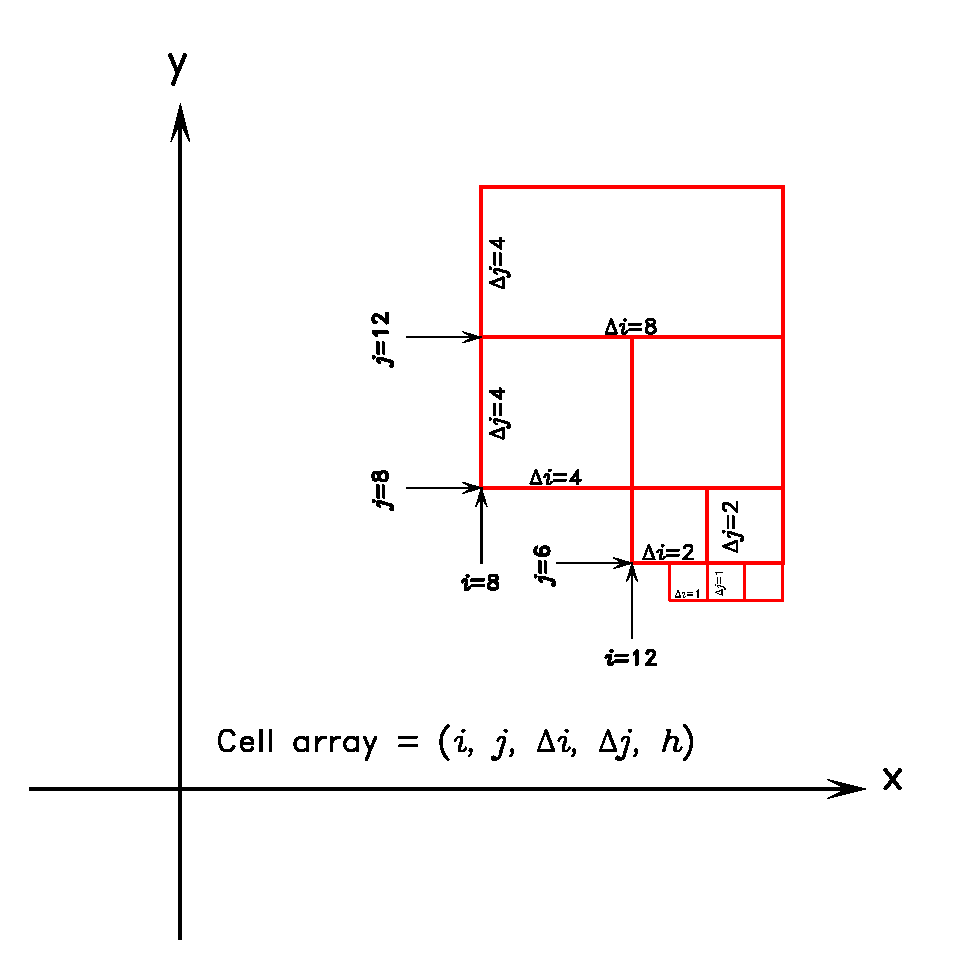
\epsfig{file=./num/smcelary.eps,angle=0,width=3.in}}
\caption{SMC 网格中使用的单元数组示意。}
\label{fig:SMCells} \botline
\end{figure}

SMC 网格的一个重要特征是它是非结构网格，也就是说，单元不要求按照其物理位置相邻排列。为便于多分辨率 SMC 网格，单元按其大小排序，使给定层级上的单元聚集在一个子循环中，共用一个子时间步。细化层级子步的基础层级时间步随网格长度一起减半。这有效避免了模式因细化单元的 CFL 限制而变慢。传播格式所需的相邻单元信息由单元面数组提供，这些面数组会针对给定单元数组列表预先计算。因此，不需要把仅含海点的 SMC 网格单元扩展到完整网格上进行传播。图~\ref{fig:SMCells} 展示了 SMC 单元数组的定义方式，图~\ref{fig:SMC_Arctic} 展示了 6-12-25 km 三层 SMC 网格中的北极区域。金色和红色圆圈分别标记 SMC6-25 网格中的全球部分和北极部分。金色圆圈内的北极部分需要固定参考方向来定义其波向箱。全球部分（直到金色圆圈）可在没有北极部分的情况下独立运行。如果用 ARC 选项激活北极部分，则从红色圆圈到金色圆圈的 4 行会在北极部分中复制为边界单元。北极部分使用单独的单元和面数组，并在波浪模式中并入全球数组用于传播。对于带输入边界条件的区域 SMC 网格，需要提供边界单元序号列表，并由 {\F PSMC} namelist 参数 {\code NBISMC} 指定边界单元数量。SMC 网格使用与规则经纬度网格相同格式的边界输入文件。边界文件可由规则网格或全球 SMC 网格模式生成，方法与规则网格一样指定边界单元中心位置。

\begin{figure}
\centerline{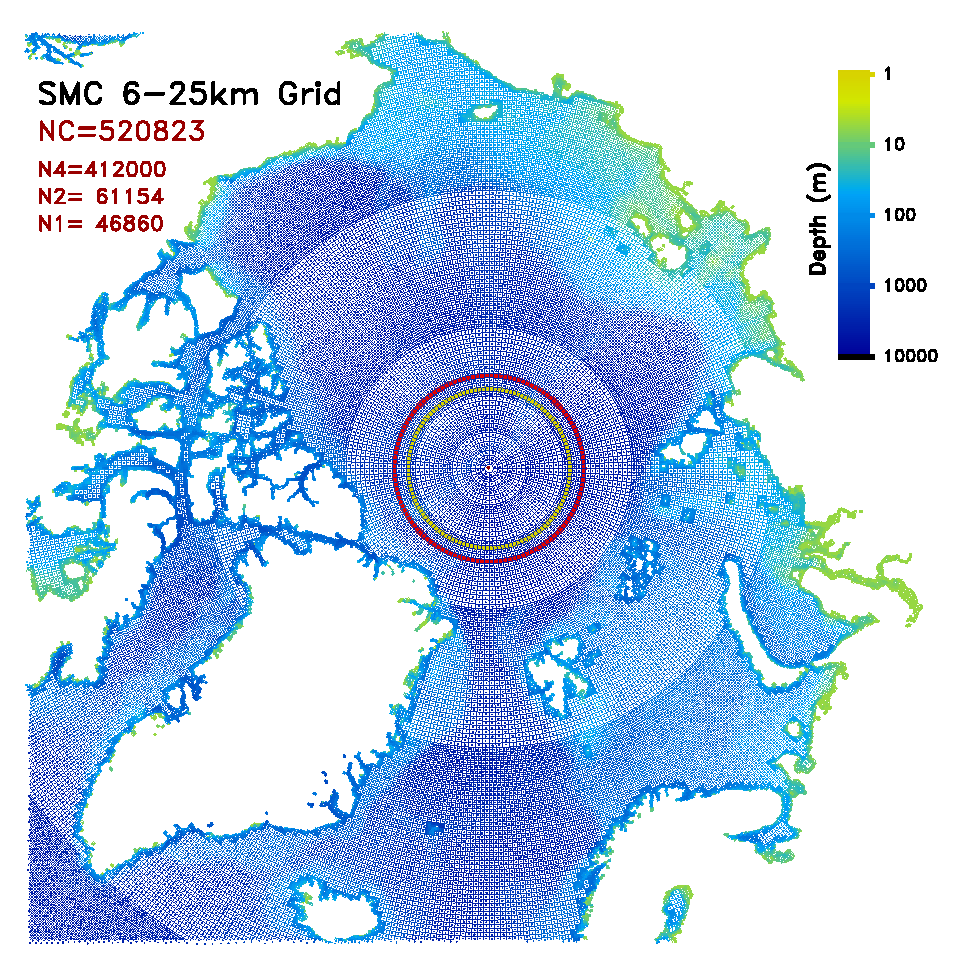
\epsfig{file=./num/JCP_Fig2_GArc.eps,angle=0,width=4.in}}
\caption{6-12-25km 多分辨率 SMC 网格中的北极区域。}
\label{fig:SMC_Arctic} 
\botline
\end{figure}

已开发若干 IDL 和 F90 程序，用于生成 SMC 网格单元和面数组，以及可视化网格网格和波场，但它们尚未正式纳入 WW3 软件包。smc\_docs/SMCG\_TKs/ 中提供了一个 IDL 程序 (Glob50SMCels.pro)，用于使用规则 50 km 网格水深文件 (G50kmBathy.dat) 生成全球 50km SMC 网格。面数组由两个 F90 程序生成，一个用于全球部分 (G50SGlSide.f90)，另一个用于北极部分 (G50SAcSide.f90)。由于极区单元的特殊处理 \citep{art:Li12}，北极极点单元的面数组需要采用不同于其他单元的方法。单元数组文件必须先用一个简单 Linux 脚本 (countcells) 排序，然后再输入面数组生成程序。面数组也需要用 Linux 脚本 (countijsd) 排序，以确定多层级子循环计数。可运行一个独立谱传播测试 (G50SMCSRGD.f90) 来测试单元和面数组，其输出可用 IDL 脚本 g50smstrspb.pro 可视化；该脚本使用 SMC 网格可视化程序 g50smcgrids.pro 保存的投影文件。通过修改 g50smcgrids.pro 中的投影参数，用户可选择投影视点（以经纬度度数表示），并保存投影供模式输出可视化使用。子网格阻挡文件可由 IDL 程序 Glob50SMCObstr.pro 生成。

SMC 网格选项的编译类似于规则经纬度网格，但需要额外开关 {\code SMC} 来调用 SMC 网格。由于 SMC 网格与规则经纬度网格共享若干网格变量，也应选择规则网格开关，例如 {\code PR2 UNO} 或 {\code PR3 UQ}。SMC 网格类型 {\code SMCTYPE} 通过在 ww3\_grid.inp 文件中用 {\code SMCG} 替换 {\code RECT} 来定义。注意，SMC 网格构建在规则经纬度网格内部，因此在 ww3\_grid.inp 文件中仍需基础分辨率层级上的规则经纬度网格参数，如 NX、NY、SX、SY、X1 和 Y1。规则经纬度网格水深、陆海掩膜和子网格阻挡输入文件不再需要，它们由 SMC 网格仅海点文件替代（水深存储在单元数组中，子网格阻挡存储在 G50GObstr.dat 中）。不过，ww3\_grid.inp 中的水深和陆海掩膜输入行会保留，用于传递最小水深等参数。由于高纬度处的合并以及可能存在的细化分辨率，规则网格映射数组会为与 SMC 网格单元保持一致而略作修改。三层 Lake Erie SMC 网格模式示例见回归测试 \emph{regtests/ww3\_tp2.10}。

SMC 网格模式的输出后处理已针对 ww3\_ounf 和 ww3\_outf 开发。对于 ww3\_ounf，用户可选择在原生模式网格海点上提取多分辨率信息，或在模式网格定义中设置的任一分辨率层级上生成规则网格。ww3\_outf 程序处理 SMC 网格数据时，可输出为基础分辨率层级上完全展开的规则经纬度网格输出，也可输出为所有 SMC 网格海点处的 ASCII 输出（type-4）。对于规则网格输出，参数值由所有与所选输出单元边界重叠的 SMC 网格单元作面积加权平均确定。海点数据的纬度和经度对应原生模式网格单元中心。对于 ww3\_ounf 海点输出，netCDF 文件中还提供描述单元大小的变量。

本代码版本未提供海点输出的可视化工具；不过，可根据请求从 Met Office 获得一些示例。针对 netCDF 海点输出，已开发一个基于 python 的 GUI 工具。所有单元 ASCII 输出可借助输入单元数组文件进行可视化，因为输出单元顺序与输入单元数组相同。IDL 脚本 g50smcswhglb.pro 是绘制全球 50km SMC 网格 SWH 输出的示例程序。它使用 g50smcgrids.pro 生成的投影文件。鼓励用户用其他语言开发自己的网格生成和后处理程序。一个 Python 小组已经成立，用于开发 SMC 网格单元和面数组生成及可视化程序。这些新的 Python 程序目前存放在一个单独的 github 站点：  
\url{https://github.com/ww3-opentools/ww3-grid/}
该站点仍处于开发阶段。欢迎 WW3 Python 程序员测试并为其改进作贡献。

从第 7 版起，SMC 网格扩展为可在 WW3 多网格模式下运行。目前，它只支持同等级 SMC 子网格并行运行。SMC 子网格的生成方式类似于具有自身边界单元列表的单个区域 SMC 网格。建议边界单元采用来自相邻子网格的复制单元，因为 SMC 子网格的边界谱交换为整谱复制粘贴，即不需要插值。规则经纬度子网格也可加入同一等级的 SMC 子网格组，但边界条件仍限于整谱交换。原始经纬度网格边界插值未启用。该简化减少了 MPI 通信负载，但如果边界单元中心未对齐，可能会损失一些精度。Great Lakes 的 SMC 子网格示例见回归测试 \emph{regtests/mww3\_test\_09}。它以 3 个 SMC 层级（0.5-1-2 km）覆盖 Lake Michigan、Huron 和 Superior，并尽量减少边界连接。
  
SMC 网格支持混合并行化；在 Cray XC40 超级计算机上使用 3 或 6 个 OpenMP 线程运行时，总耗时可减少一半。进一步增加 OpenMP 线程似乎效果不大。混合并行和多网格并行相结合，可使 \emph{mww3\_test\_09} 中 3 个 Great Lake 子网格的计算机使用规模扩展到 100 个以上节点。

建议阅读 smc\_docs/SMC\_Grid\_Guide.pdf 或会议网页上的会议论文 \citep{tol:LiS17}：
http://www.waveworkshop.org/15thWaves/
以获取更多信息；关于 SMC 网格的任何帮助，也可联系 \url{Jian-Guo.Li@metoffice.gov.uk}。


\vsssub
\subsubsection{~Garden Sprinkler Effect} \label{sub:num_GSE}
\vsssub

\noindent
高阶精度传播格式的数值扩散足够小，因此可能出现所谓的 “Garden Sprinkler Effect”（GSE）：也就是说，由于谱的离散描述，连续涌浪场会分解为一组离散涌浪场 \citep[图~3c]{art:BH87}。\ws\ 中提供了若干 GSE 缓解方法，如以下各节所述。

\addcontentsline{toc}{subsubsection}{\strut \hspace{24mm} 不进行 GSE 缓解}

\vspace{\baselineskip}
\vspace{\baselineskip}
\noindent {\bf 不进行 GSE 缓解}

\opthead{PR0 / PR1}{\ws}{H. L. Tolman}

\noindent
在无传播（开关 {\code PR0}）的情况下，或在传统网格或曲线网格中使用一阶传播格式时，既没有可用的 GSE 缓解方法，也不需要进行 GSE 缓解。

\pb
\addcontentsline{toc}{subsubsection}{\strut \hspace{24mm} Booij and Holthuijsen 1987}

\vspace{\baselineskip} 
\vspace{\baselineskip} 
\noindent {\bf Booij and Holthuijsen 1987}

\opthead{PR2}{\ws}{H. L. Tolman}


经典 GSE 缓解方法来自 \cite{art:BH87}。他们为离散谱推导了另一种传播方程，其中包含扩散修正，以便在谱描述离散的情况下仍能考虑连续色散。该修正只影响空间传播；对于一般空间坐标 $(x,y)$，其形式为

% ------ Correction linear dispersion --------- %
% eq:d_bal_0         Booij and Holthuijsen, 1987
% eq:Dxx
% eq:Dyy
% eq:Dxy
% eq:Dss
% eq:Dnn

\begin{equation}
\frac{\p \cN}{\p t} +
\frac{\p}{\p x} \left [ \dot{x} \cN 
           - D_{xx} \frac{\p \cN}{\p x} \right ] +
\frac{\p}{\p y} \left [ \dot{y} \cN 
           - D_{yy} \frac{\p \cN}{\p y} \right ] -
2 D_{xy} \frac{\p^2 \cN}{\p x \p y} = 0
\: , \label{eq:d_bal_0}\end{equation}  \begin{equation}
D_{xx} = D_{ss} \, \cos^2 \theta + D_{nn} \, \sin^2 \theta
\: , \label{eq:Dxx} \end{equation} \begin{equation}
D_{yy} = D_{ss} \, \sin^2 \theta + D_{nn} \, \cos^2 \theta
\: , \label{eq:Dyy} \end{equation}  \begin{equation}
D_{xy} = ( D_{ss} - D_{nn} ) \, \cos \theta \, \sin \theta
\: , \label{eq:Dxy} \end{equation} \begin{equation}
D_{ss} = (\Delta c_g )^2 \: T_s / 12
\: , \label{eq:Dss} \end{equation} \begin{equation}
D_{nn} =  ( c_g \Delta \theta )^2 \: T_s / 12
\: , \label{eq:Dnn} \end{equation}

\noindent
其中 $D_{ss}$ 是离散波分量传播方向上的扩散系数，$D_{nn}$ 是沿该离散波分量波峰方向的扩散系数，$T_s$ 是自涌浪生成以来经过的时间。在当前分步法中，扩散可作为单独步骤加入：

% eq:d_bal_1         Separated diffusion equation

\begin{equation}
\frac{\p \cN}{\p t} = 
\frac{\p}{\p x} \left [ D_{xx} \frac{\p \cN}{\p x} \right ] +
\frac{\p}{\p y} \left [ D_{yy} \frac{\p \cN}{\p y} \right ] +
   2 D_{xy} \frac{\p^2 \cN}{\p x \p y}
\: . \label{eq:d_bal_1} \end{equation}

\noindent
该方程在实现时采用两个简化，其合理性见 \cite{tol:OMB95} 的讨论。第一，涌浪“年龄” $T_s$ 在整个模式中保持常数（由用户定义，没有默认值）。第二，扩散系数 $D_{ss}$ 和 $D_{nn}$ 按深水假设计算：

% eq:Dss_d
% eq:Dnn_d

\begin{equation}
D_{ss} = \left ( \: (X_\sigma-1) \: \frac{\sigma_m}{2 k_m} \right )^2
\: \frac{T_s}{12} \: , \label{eq:Dss_d} \end{equation} \begin{equation}
D_{nn} =  \left ( \frac{\sigma_m}{2 k_m} \Delta \theta \right )^2
\: \frac{T_s}{12} \: , \label{eq:Dnn_d} \end{equation}

\noindent
其中 $X_\sigma$ 按式~(\ref{eq:sigma_grid}) 定义。采用这两个假设后，对于每个独立谱分量，扩散张量在整个空间区域内为常数。

式~(\ref{eq:d_bal_1}) 用前向时间、中心空间格式求解。在 $\phi$ ($x$) 空间中点 $i$ 与 $i-1$ 之间的单元界面处，式~(\ref{eq:d_bal_1}) 右端第一项中方括号内的项（记为 $\cD_{i,-}$）估计为

% eq:ddif_1          Discrete diffusion 1

\begin{equation}
D_{xx} \frac{\p \cN}{\p x} \approx \cD_{i,-} =
\left . D_{xx} \; \left ( \frac{\cN_i - \cN_{i-1}}{\Delta x} \right ) \: 
\right |_{j,l,m} \: . \label{eq:ddif_1} \end{equation}

\noindent
计数器为 $i$ 和 $i+1$ 的相应值，以及 $\lambda$ ($y$) 空间中的梯度，仍通过轮换索引和增量得到。如果两个网格点之一位于陆地上，则式~(\ref{eq:ddif_1}) 设为零。式~(\ref{eq:d_bal_1}) 右端的混合导数（记为 $\cD_{ij,--}$）在 $x$ 空间中的网格点 $i$ 和 $i-1$、以及 $y$ 空间中的 $j$ 和 $j-1$ 上估计为

% eq:ddif_2          Discrete diffusion 2

\begin{equation}
\cD_{ij,--} = \left . \: D_{xy} 
\left ( \frac{- \cN_{i,j} + \cN_{i-1,j} +
              \cN_{i,j-1} - \cN_{i-1,j-1}}
           {0.5 ( \Delta x_j + \Delta x_{j-1} ) \: \Delta y}
              \right ) \: \right |_{l,m} 
\: . \label{eq:ddif_2} \end{equation}

\noindent
注意，由于使用球面网格，增量 $\Delta x$ 是 $y$ 的函数。只有当所考虑的四个网格点全为海点时才计算该项，否则将其设为零。对式~(\ref{eq:d_bal_1}) 中第一项采用时间前向离散，对右端第一项和第二项的其余部分采用空间中心离散，最终算法为

% eq:ddif_3          Discrete diffusion 3

\begin{eqnarray}
\cN_{i,j,l,m}^{n+1} = \cN_{i,j,l,m}^n + 
\frac{\Delta t}{\Delta x} 
   \left ( \cD_{i,+} - \cD_{i,-} \right ) +
\frac{\Delta t}{\Delta y}
   \left ( \cD_{j,+} - \cD_{j,-} \right ) \nonumber \\
+ \frac{\Delta t}{4} \left ( \cD_{ij,--} + 
   \cD_{ij,-+} + \cD_{ij,+-} + \cD_{ij,++} \right )
\: . \label{eq:ddif_3} \end{eqnarray}

\noindent
当满足下式时可得到稳定解 \citep[e.g.,][Part I section 7.1.1]{bk:Fle88}：

% eq:ddif_4          Stability

\begin{equation}
\frac{D_{\max} \: \Delta t}{\min(\Delta x , \Delta y)^2}
\leq 0.5 \: , \label{eq:ddif_4} \end{equation}

\noindent
其中 $D_{\max}$ 为扩散系数的最大值（通常 $D_{\max} = D_{nn}$）。由于该稳定性判据是网格增量的二次函数，在大尺度应用的高纬度地区，稳定性可能成为严重问题。为避免这对模式时间步长造成过度约束，使用修正涌浪年龄 $T_{s,c}$：

% eq:Ts_cor

\begin{equation}
T_{s,c} = T_s \min \left \{ \: 1 \: , \: 
\left ( \frac{\cos(\phi)}{\cos(\phi_c)} \right )^2 \: \right \}
\: , \label{eq:Ts_cor} \end{equation}

\noindent
其中 $\phi_c$ 是用户定义的截止纬度。

\vspace{\baselineskip} \noindent
 
上述扩散是涌浪传播所需要的，但对增长中的风海并不真实。对于风海，不带色散修正的 \uq{} 格式已经足够平滑，可以给出稳定的有限风区增长曲线 \citep{tol:OMB95}。为去除轻微振荡，对增长中的波分量使用小的各向同性扩散。为保证该扩散较小且对所有谱分量等效，它由预设的单元 Reynolds（或单元 Peclet）数 $\cR = c_g \Delta x D_g^{-1} = 10$ 计算，其中 $D_g$ 是增长分量的各向同性扩散：

% eq:Dg              Diffusion growing components

\begin{equation}
D_g = \frac{c_g \: \min(\Delta x , \Delta y)}{\cR} \: . \label{eq:Dg}
 \end{equation}

\noindent
涌浪和风海的扩散按无量纲风速或反波龄 $u_{10} c^{-1} = u_{10} k \sigma^{-1}$ 进行线性组合：

% eq:Xg              Linear combination for diffusion
% eq:Dss_f           Final Dss
% eq:Dnn_f           Final Dnn

\begin{equation}
X_g = \min \: \left \{ \: 1 \: , \: \max \: \left [ \: 0 \: , \:
3.3 \left ( \frac{k \, u_{10}}{\sigma} \right ) - 2.3
\: \right ] \: \right \}
 \: , \label{eq:Xg} \end{equation} \begin{equation}
D_{ss} = X_g D_g + (1-X_g) D_{ss,p}
\: , \label{eq:Dss_f} \end{equation} \begin{equation}
D_{nn} = X_g D_g + (1-X_g) D_{nn,p}
\: , \label{eq:Dnn_f} \end{equation}

\noindent
其中后缀 $p$ 表示式~(\ref{eq:Dss_d}) 和 (\ref{eq:Dnn_d}) 中定义的传播扩散。式~(\ref{eq:Dg}) 和 (\ref{eq:Xg}) 中的常数在模式中预设。


\pb
\addcontentsline{toc}{subsubsection}{\strut \hspace{24mm} 空间平均}

\vspace{\baselineskip} 
\vspace{\baselineskip} 
\noindent {\bf 空间平均}

\opthead{PR3}{\ws}{H. L. Tolman}


上述 GSE 缓解方法的主要缺点，是它可能影响模式经济性；这与式~(\ref{eq:ddif_4}) 有关，并在 \cite{tol:Waves01a,tol:OMOD02b} 中有讨论。因此，\ws\ 又开发了一种替代的附加 GSE 缓解方法。

该方法是 \ws\ 的默认方法，它用一个单独的分步替代附加扩散步骤 (\ref{eq:d_bal_1})；在该分步中，对给定谱分量的能量密度场进行直接平均。每个网格点周围用于平均的区域，在传播方向 ($\bs$) 和法向方向 ($\bn$) 上分别延伸为

\begin{equation}
\pm \gamma_{a,s} \: \Delta c_g \: \Delta t \: \bs \:\:\: ,
\pm \gamma_{a,n} \: c_g \Delta \theta \: \Delta t \: \bn \:\:\: , \label{eq:GSE_avg}
\end{equation}

\noindent
其中 $\gamma_{a,s}$ 和 $\gamma_{a,n}$ 为可调常数，默认值设为 1.5。该平均过程如图~\ref{fig:GSE_1} 所示。注意，如 \cite{tol:OMOD02b} 所讨论，在实际应用中这些值可能需要重新调整。该文附录 A 给出了平均格式的细节，包括守恒性方面的考虑。此外，与 \cite{art:BH87} 方法保持一致意味着 $\gamma_{a,s}$ 和 $\gamma_{a,n}$ 应随空间网格分辨率变化 \citep[见][Appendix]{tol:OMOD08a}。

注意，具有主导方向 $\bs$ 和 $\bn$ 的这种平均类似于 \cite{art:BH87} 的扩散方法，后者使用相同主方向。然而，该平均方法绝不会影响时间步长，因为它与实际传播完全分离。此外，如果使用显式格式，通常有 $c_g \Delta t / \Delta x < 1$，那么显然按 (\ref{eq:GSE_avg}) 定义的区域进行平均，一般只需要直接相邻空间网格点的信息，如图~\ref{fig:GSE_1} 所示。此外，该方法不需要高纬度滤波。

\begin{figure} \begin{center}
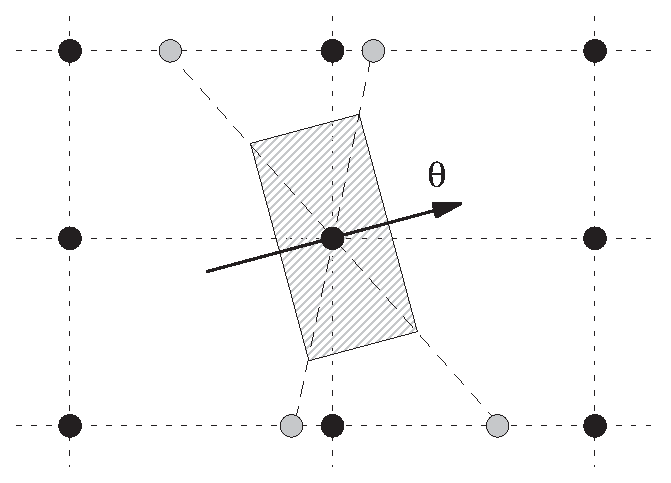
\epsfig{file=./num/GSE_1.eps,angle=0,width=2.2in}
\caption{空间平均 GSE 缓解技术示意图。实心圆和虚线表示空间网格。阴影区域表示需要考虑的平均区域。角点值由中心网格点和灰色点得到；后者通过相邻网格点插值得到 \citep[引自][]{tol:OMOD02b}。}
\label{fig:GSE_1} \botline
\end{center}
\end{figure}

如 \cite{tol:OMOD02b,tol:OMB02b} 所示，该方法给出的结果几乎与前一种方法相同，但计算成本略低。对于高分辨率应用，平均方法可能显著更经济。



最后，通过保证离散谱方向不与空间网格线重合，也可在一定程度上缓解 GSE。这可通过把第一个离散方向 $\theta_1$ 定义为

% eq:theta1          First direction

\begin{equation}
\theta_1 = \alpha_\theta \: \Delta \theta \:\:\: , \label{eq:theta1}
\end{equation}

\noindent
其中 $-0.5 \leq \alpha_\theta \leq 0.5$ 可由用户定义。注意，设置 $\alpha \neq 0$ 有利于一阶格式，但对三阶格式影响可忽略。
 

\pb
\vsssub
\subsubsection{~未解析障碍物} \label{sub:num_obst}
\conthead{\ws}{H. L. Tolman, L. Mentaschi}

\noindent
即使在 \ws\ 1.15 版最初调参时 \citep{tol:OMB02a}，也已清楚未解析岛群是局地波浪模式误差的主要来源。这一点在 \citet[][图~3]{tol:Waves01a} 和 \citet[][图~8]{tol:WaF02} 中有更详细说明。在 \ws\ 中，有两种方法可用于参数化未解析障碍物。第一种方法最初来自 \swan\ \citep{art:BRH99,man:SWAN3}，它在数值格式内部的空间网格单元边界处施加未解析障碍物的影响，并已用于规则网格。第二种方法由 \citep{art:Mentaschi2015b} 提出，基于源项，可应用于不同网格类型。本节介绍第一种方法；第二种方法的说明见第 \ref{sec:UOST} 节。

在基于传播的方法中，通过单元公共边界的数值通量会按照未解析障碍物提供的阻挡程度受到抑制。在该方法中，式~(\ref{eq:uq_xy_tot}) 的 \uq{} 格式数值传播格式修改为

% eq:uq_xy_obstr

\begin{equation}
\cN_{i,j,l,m}^{n+1} = \cN_{i,j,l,m}^n +
\frac{\Delta t}{\Delta \phi} \left [ \alpha_{i,-} \cF_{i,-} - \alpha_{i,+} \cF_{i,+} \right ]
\: , \label{eq:uq_xy_obstr} \end{equation}

\begin{figure} \begin{center}
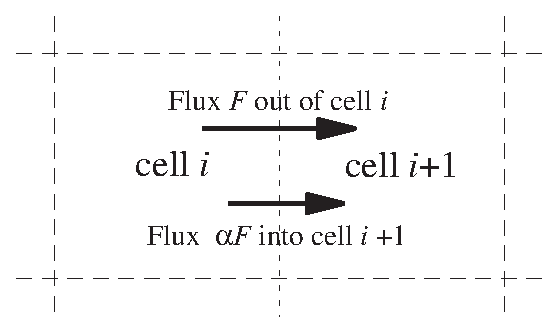
\epsfig{file=./num/obstr.eps,angle=0,width=2.2in}
\caption{未解析障碍物的处理。公共单元边界（点线）的透明度为 $\alpha$。虚线表示其他单元边界。数值通量从左向右。}
         \label{fig:obstr} \botline
\end{center}
\end{figure}

\noindent
其中 $\alpha_{i,-}$ 和 $\alpha_{i,+}$ 是相应单元边界的“透射率”，范围从 0（封闭边界）到 1（无遮挡）。对于出流边界，透明度按定义为 1，否则能量会在单元中人为累积。对于入流边界，小于 1 的透明度会导致受阻能量在单元边界处被移除。该方法如图~\ref{fig:obstr} 所示。注意，类似方法很容易应用于一阶和二阶格式。还需注意，\cite{art:HY96} 和 \cite{art:HMM00} 曾使用另一种障碍物方法，其中障碍物是谱方向 $\theta$ 的函数。

模式中有两种定义障碍物的方法。第一种方法直接在网格边界处定义障碍物。这需要生成交错的水深-透明度网格。第二种方法允许用户在同一网格上定义水深和透明度。在这种情况下，入流边界处的透明度为 $0.5(1+\alpha_i)$，而出流透明度按定义为 1。为完成总透明度 $\alpha_i$，流向上的下一个单元将具有入流透明度 $2\alpha_i/(1+\alpha_i)$。如果连续单元均部分受阻，则采用各个透明度的乘积。

该方法也可用于连续模拟冰覆盖对波浪传播的影响。这一点在 \para\ref{sub:num_ice} 中讨论。岛屿和海冰的子网格处理细节见 \cite{tol:OMOD03a}。该方法在大尺度波浪模式中的影响研究见 \cite{tol:OMB02b,tol:OMOD03a}。

\ws\ 的默认设置是不包括障碍物的子网格建模。生成阻挡网格可能非常耗费人力。因此，\cite{tol:MMAB07a, tol:OMOD08a} 开发了一种自动生成海底和阻挡网格的方法。注意，该选项不涉及编译级选择，而完全由网格预处理器控制（见第 \ref{chapt:run} 章）。


\vsssub
\subsubsection{~连续移动网格} \label{sub:num_move}
\opthead{MGx}{\ws}{H. L. Tolman}

\addcontentsline{toc}{subsubsection}{\strut \hspace{24mm} 一般概念}


为处理飓风等快速变化、小尺度条件下的波浪增长问题，模式 3.02 版加入了一个选项，可向网格添加给定的连续平流速度。该模式版本在 \cite{tol:OMOD05b} 中有详细说明。这里仅给出简要描述。



\begin{center}
\rule[1mm]{55mm}{1.0mm} WARNING \rule[1mm]{55mm}{1.0mm} \\
 \vspace{\baselineskip}
\parbox{120mm}{\ws\ 的连续移动网格版本仅用于在高度理想化条件下测试波浪模式性质。该模式版本只应在无平均流、无陆块的深水条件下使用。此外，为避免大圆传播带来的复杂性，只应使用 Cartesian 网格。该选项也仅针对传播选项 {\F pr1} 和 {\F pr3} 实现。注意，无论在编译阶段还是运行阶段，脚本或程序都不会检查这些条件。该选项不被视为适合一般应用。} \\
\vspace{\baselineskip}
\rule[1mm]{55mm}{1.0mm} WARNING \rule[1mm]{55mm}{1.0mm}
\end{center}

\noindent
对于上述应用，式~(\ref{eq:bal_plane}) 可写为

\begin{equation}
\frac{\partial N}{\partial t} + 
\left ( {\bf\dot{x}}-{\bf{v}}_g \right ) \cdot \nabla_x N  = 
\frac{S}{\sigma} \: , \label{eq:bal_move}
\end{equation}

\noindent
其中 ${\bf{v}}_g$ 表示网格的平流速度。该选项在编译模式时选择。第二个编译级选项允许把网格平流速度 ${\bf{v}}_g$ 加到风场上。这样提供了一种简单方法，可保证风场质量守恒不依赖于实际和瞬时的网格平流速度。平流速度 ${\bf{v}}_g$ 可随时间变化，并由用户在模式运行时提供（见下文）。




在式~(\ref{eq:bal_move}) 适用的简化条件下，如果考虑到该方程等价于

\begin{equation}
\frac{\partial N}{\partial t} + 
\nabla_x \cdot \left ( {\bf\dot{x}}-{\bf{v}}_g \right ) N  = 
\frac{S}{\sigma} \: , \label{eq:bal_move2}
\end{equation}

\noindent
则移动网格的实现很直接。这又意味着，对于求解式~(\ref{eq:bal_plane}) 的任意数值格式，平流速度 ${\bf{v}}_g$ 可直接加到 ${\bf\dot{x}}$ 中。由于这会影响净平流速度，也会影响稳定性特征。该影响已通过在式~(\ref{eq:dtpl}) 的实际传播时间步长计算中包含移动网格速度而自动考虑。因此，用户只需提供代表 $\bf{v}_g = 0$ 情形的合适最大传播时间步长。

由于频率相同但传播方向不同的谱分量在网格中的停留时间不同，网格运动会对 Garden Sprinkler Effect (GSE) 产生表观影响。当前 GSE 缓解方法对较年轻涌浪往往比对较老涌浪更有效。因此，在移动网格中停留时间较长的涌浪往往表现出更明显的 GSE \citep[见][]{tol:OMOD05b}。为缓解 GSE 缓解中的这种表观不平衡，将式~(\ref{eq:GSE_avg}) 替换为

\begin{equation}
\pm \gamma_a \gamma_{a,s} \: \Delta c_g \: \Delta t \: \bs \:\:\: ,
\pm \gamma_a \gamma_{a,n} \: c_g \Delta \theta \: \Delta t \: \bn \:\:\: ,
\label{eq:move_GSE_avg1}
\end{equation}

\begin{equation}
\gamma_a = \left ( \frac{|\dot{\bf{x}}|}{|\dot{\bf{x}}-\bf{v}_g|}
\right ) ^{p}
\label{eq:move_GSE_avg2}
\end{equation}

\noindent
其中 $\gamma_a$ 是考虑网格运动的修正因子，幂次 $p$ 是允许一定调节的参数。采用该修改后，可根据相应谱分量在移动网格中的预期停留时间，重新缩放所施加的平滑量，从而使 GSE 影响在网格上分布得更均匀 \citep[见][]{tol:OMOD05b}。


为开启移动网格选项或风场/GSE 修正，在 \ws\ 源代码中加入了三个可选开关（另见 \para\ref{sec:switches}）：

\begin{slist}
\sit{mgp} {Apply advection correction for continuous moving grid.}
\sit{mgw} {Apply wind correction for continuous moving grid.}
\sit{mgg} {Apply GSE alleviation for
           continuous moving grid.}
\end{slist}

\noindent
平流速度和方向输入到 shell 的方式类似于均匀流输入（见第~\ref{sec:ww3shel} 节中 {\file ww3\_shel.inp} 文件底部），只是把关键字 `{\code CUR}' 换为 `{\code MOV}'。与所有均匀输入场一样，平流速度可随时间变化。移动网格模式运行示例见测试算例 {\file ww3\_ts3}。第 \ref{sec:ww3multi} 节中的 {\file ww3\_multi.inp} 也有类似能力，并在测试算例 {\file mww3\_test\_05} 中测试。

\vssub
\subsubsection{~旋转网格} \label{sub:num_space_rotagrid}
\opthead{RTD}{\ws\ (MetOffice)}{J.-G. Li}

\noindent
旋转网格是一种纬度-经度（lat-lon）网格，通过沿经度 $\lambda_{p}$ 旋转北极，使其在标准纬度-经度系统中移到纬度 $\phi_{p}$ 的新位置得到。选择新的极点位置，是为了可将目标模式区域放在旋转赤道区域附近，从而得到间距更均匀的经纬度网格。因此，旋转网格也称为\emph{赤道网格}。例如，UK Met Office 使用的 North Atlantic and European wave (NAEW) 模式采用位于 37.5N、177.5E 的旋转极点，使英国伦敦（\textasciitilde{}51.5N 0.0E）几乎位于旋转赤道上。与同一区域中的标准经纬度网格相比，该旋转网格可在 NAEW 区域内提供间距均匀得多的经纬度网格。

在 \ws\ 中，旋转网格以对原始经纬度网格最小修改的方式实现。实际上，在模式内部旋转网格的处理就像标准经纬度网格一样。若要建立并运行旋转网格模式配置，用户应选择规则经纬度网格并使用 {\code RTD} 开关。旋转极点位置通过输入文件 {\bf ww3\_grid.inp} 中 {\code ROTD} namelist 下的 {\code PLAT} 和 {\code PLON} 变量设置（见第~\ref{sec:config011} 节）。如果极点设置为 {\code PLAT = 90.0}、{\code PLON = -180.0}，则该网格按标准经纬度系统处理。

风、流和冰文件等模式输入文件应映射到旋转网格上。为方便在标准经纬度网格框架中嵌套，提供给旋转网格以及从旋转网格输出的边界条件数据，使用以标准网格北向为参考的谱和标准经纬度网格点值；这些值会在 \ws\ 内部转换为旋转网格经纬度。{\bf ww3\_shel.inp} 或 {\bf ww3\_shel.nml} 中的二维谱输出位置列表也用标准经纬度指定。

当从标准网格嵌套到旋转网格模式时，外层和内层网格对应的模式可执行文件都应在编译时设置 {\code RTD} 开关。当从旋转网格嵌套到标准网格模式时，内层（标准）网格模式不需要用 {\code RTD} 编译。

输出到单向嵌套内层网格边界点的谱按附录~\ref{app:nest} 所述传递。输出边界条件在输入文件中定义（见 {\bf ww3\_grid.inp}，第~\ref{sec:config011} 节），形式为以内层网格坐标给出的一系列直线。如果内层网格为旋转网格，则其极点位置必须在外层网格的 {\code ROTB} namelist 下定义为数组元素 {\code BPLAT(\sl{n})} 和 {\code BPLON(\sl{n})} 的值。数组索引 {\sl{n}} 是边界条件文件 {\file nest{\sl{n}}.ww3} 的索引（{\sl{1:9}}）。

旋转网格的模式方向输出和 x-y 矢量输出可通过把 {\bf ww3\_grid.inp} 的 ROTD namelist 中 UNROT 变量设为 True，转换为标准网格北向参考。采用该设置后，对于点输出经纬度位置，所有方向值如风向、流向和二维谱都会转换为标准经纬度取向。用于反旋转网格化场的函数应用在 {\bf ww3\_ounf}、{\bf ww3\_outf} 和 {\bf ww3\_grib} 中。运行 {\bf ww3\_ounf} 和 {\bf ww3\_ounp} 时，生成的 netCDF 文件将包含变量属性 direction\_reference，用于说明使用的是标准（真北）方向参考系还是旋转网格方向参考系。由 {\bf ww3\_ounf} 生成的网格化 netCDF 文件还包含 \emph{standard\_latitude} 和 \emph{standard\_longitude} 二维数组，用于描述旋转模式单元中心在标准经纬度参考系中的位置。

如果用户希望使用 {\bf ww3\_bound} 或 {\bf ww3\_bounc} 边界处理程序为旋转极点网格生成边界条件，需要注意这些程序的输入谱始终预期在\emph{标准极点}上表述。

模块 {\bf w3servmd.ftn} 中提供了六个用于旋转网格转换的子程序：
\begin{vlist}
\vit{w3spectn}{}{Turns wave spectrum anti-clockwise by AnglD}
\vit{w3acturn}{}{Turns wave action(k,nth) anti-clockwise by AnglD}
\vit{w3thrtn}{}{Turns direction parameters anti-clockwise by AnglD}
\vit{w3xyrtn}{}{Turns x-y vector parameters anti-clockwise by AnglD}
\vit{w3lltoeq}{}{Convert standard into rotated lat/lon plus AnglD}
\vit{w3eqtoll}{}{Reverse of w3lltoeq, but AnglD unchanged}
\end{vlist}
这些子程序是自包含的，可从模式中提取出来，用于旋转网格文件的前处理或后处理。已有一些基于这些子程序开发的转换工具，但尚未包含在 \ws\ 中。旋转网格模式（NAEW）的示例见回归测试 \emph{regtests/ww3\_tp2.11}。用户可在 \emph{smc\_docs/Rotated\_Grid.pdf} 中找到更多信息，或联系 Jian-Guo Li 获取帮助（\url{Jian-Guo.Li@metoffice.gov.uk}）。

\vssub
\subsection{~谱内传播} \label{sub:spec}
\vssub
\subsubsection{~一般概念}
\vsssub

数值分步算法的第三步考虑折射和残余（流致）波数偏移。无论空间网格离散和坐标系统如何，该步骤中要求解的方程为

%-----------------------------------%
% Step : Intra-spectral propagation %
%-----------------------------------%
% eq:step_intra
% eq:k_dot_g

\begin{equation}
\frac{\p N}{\p t} + \frac{\p}{\p k} \, \dot{k}_g N +
\frac{\p}{\p \theta} \, \dot{\theta}_g N = 0
\: , \label{eq:step_intra} \end{equation} \begin{equation}
\dot{k}_g  = \frac{\p \sigma}{\p d} 
    \frac{{\bf U} \cdot \nabla_x d}{c_g}  -
    {\bf k} \cdot \frac{\p {\bf U}}{\p s}
\: , \label{eq:k_dot_g} \end{equation}

\noindent
其中 $\dot{k}_g$ 是相对于网格的波数速度，$\dot{\theta}_g$ 由 (\ref{eq:theta_g_dot}) 和 (\ref{eq:theta_dot}) 给出。该方程在 $\theta$ 空间中不需要边界条件，因为模式按定义使用完整（闭合）的方向空间。然而，在 $k$ 空间中需要边界条件。在低波数处，假定离散区域之外不存在波作用量。因此，假定在离散低波数边界处没有作用量进入模式。在高波数边界处，跨离散边界的输运按式~(\ref{eq:tail_N_k}) 给出的参数化谱形计算。计算 $\dot{\theta}$ 时所需的水深导数主要使用中心差分确定。不过，对于靠近陆地的点，只使用海点的一侧差分。

$\theta$ 空间中的传播可能在显式数值格式中造成实际问题，因为对于极浅水中的长波，或由于强流切变，折射速度可能变得极大。类似地，$k$ 空间中的传播在极浅水中也会遇到类似问题。为避免因折射而需要极小时间步长，对 $\theta$ 空间和 $k$ 空间中的传播速度 (\ref{eq:theta_dot}) 进行滤波：

% eq:theta_filter

\begin{equation}
\dot{\theta} = X_{rd}(\lambda,\phi,k)\left( \dot{\theta_d} + 
\dot{\theta_c} + \dot{\theta_g} \right)\: , \label{eq:theta_filter} \end{equation}

\noindent
其中下标 $d$、$c$ 和 $g$ 分别指 (\ref{eq:theta_dot}) 中折射速度与水深、流和大圆相关的部分。滤波因子 $X_{rd}$ 对每个波数和位置分别计算，并被确定为使由\emph{水深}折射项导致的 $\theta$ 空间传播 \cfl{} 数不超过预设（用户定义）值（默认 0.7）。这对应于对某些低频波分量减小海底坡度。对于中纬度，受影响分量预期携带很少能量，因为它们位于极浅水中。携带显著能量的长波分量通常正向海岸传播，其能量无论如何都会被耗散。该滤波对短波以及靠近极点处也很重要。可通过减小谱内折射时间步长，并查看模式输出中的最大 CFL 数来测试该滤波的影响。这些最大 CFL 数在滤波应用之前计算。

% \vspace{\baselineskip}
% \centerline{\ldots ADD DYNAMIC TIME INTEGRATION \ldots}


为适应非线性相互作用 $S_{nl}$ 的计算，谱空间始终采用常数方向增量和对数频率网格 (\ref{eq:sigma_grid}) 离散。可使用一阶、二阶和三阶格式，并在以下各节介绍。

\vssub
\subsubsection{~一阶格式}
\opthead{PR1}{\ws}{H. L. Tolman}

\noindent
在一阶格式中，$\theta$ 和 $k$ 空间中的通量使用式~(\ref{eq:1up_xy_1}) 至 (\ref{eq:1up_xy_3}) 计算（将 $\cN$ 替换为 $N$，并轮换相应计数器）。完整的一阶格式为

% eq:1up_intra_tot

\begin{equation}
N_{i,j,l,m}^{n+1} = N_{i,j,l,m}^n 
 + \frac{\Delta t}{\Delta \theta} \left [ \cF_{l,-} - \cF_{l,+} \right ]
 + \frac{\Delta t}{\Delta k_m} \left [ \cF_{m,-} - \cF_{m,+} \right ]
\: , \label{eq:1up_intra_tot} \end{equation}

\noindent
其中 $\Delta \phi$ 为方向增量，$\Delta k_m$ 为（局地）波数增量。低波数边界条件通过对 $m=1$ 取 $\cF_{m,-}=0$ 施加；高波数边界条件则使用参数化近似 (\ref{eq:tail_N_k}) 计算 $N$，即把离散网格向高波数方向扩展一个网格点。

\vssub
\subsubsection{~二阶格式 (UNO)}
\opthead{UNO}{Met Office}{J.-G. Li}

\noindent
对于方向 $\theta$ 空间，UNO 格式与规则网格上的格式相同，前提是假定方向箱间距规则。然而，对于 \emph{k} 空间，UNO 格式使用其不规则版本；该版本用局地梯度而不是差分，估计谱箱 \emph{i}-1 与 \emph{i} 之间单元面中通量点处的波作用量值，即
\begin{equation}
  N_{i-}^{*}=N_{c}+sign\left(N_{d}-N_{c}\right)\frac{\left(\Delta
      k_{c}-|\dot{k}_{i-}|\Delta
      t\right)}{2}\min\left(|\frac{N_{u}-N_{c}}{k_{u}-k_{c}}|,|\frac{N_{c}-N_{d}}{k_{c}-k_{d}}|\right)
  \:\:\:,
\label{eq:UNO2irregular}
\end{equation}

\noindent
其中 \emph{i}- 为波数 \emph{k} 箱索引；下标 \emph{u}、\emph{c} 和 \emph{d} 分别表示相对于给定 \emph{i}- 面速度 $\dot{k}_{i-}$ 的\emph{上游、中心}和\emph{下游}单元；$k_{c}$ 为中心箱波数，$\Delta k_{c}$ 为中心箱宽度。不规则网格 UNO 格式的细节见 \cite{art:Li08}。

$\theta$ 空间的边界条件是自然周期条件。对于 \emph{k} 空间，由于 UNO 格式为二阶精度，在波谱区域两端各增加两个零谱箱。



\vssub
\subsubsection{~三阶格式 (UQ)}
\opthead{UQ}{\ws}{H. L. Tolman}

\noindent
$\theta$ 空间中的 \uq{} 格式采用与物理空间格式类似的方式实现，区别在于封闭的方向空间不需要边界条件。$k$ 空间中的可变网格间距需要对格式作若干修改，如 \cite[{Appendix}]{art:Leo79} 所述。于是式~(\ref{eq:quick_1}) 至
(\ref{eq:quick_4}) 变为

% ------ QUICKEST scheme for k space---------- %
% eq:quick_1k        Basic flux
% eq:quick_2k        Boundary value
% eq:quick_3k        Divergence
% eq:quick_4k        CFL number

\begin{equation}
\cF_{m,-} = \left [ \dot{k}_{g,b} \: N_b \: \right ]^n_{i,j,l}
\: , \label{eq:quick_1k}\end{equation} \begin{equation}
\dot{k}_{g,b} = 0.5 \: \left ( \dot{k}_{g,m-1} + \dot{k}_{g,m} 
\: \right )  \: , \label{eq:quick_1ak}
\end{equation} \begin{equation}
N_b = \frac{1}{2} \left [ \rule[0mm]{0mm}{\baselineskip} \: 
(1+C)N_{i-1} + (1-C)N_i \: \right ] - \:
\frac{1-C^2}{6} \: {\cal CU} \: \Delta k^2_{m-1/2}, \label{eq:quick_2k} \end{equation} \begin{equation}
{\cal CU} =  \left \{ \begin{array}{ccc}
\frac{1}{\Delta k_{m-1}}
\left [ \frac{N_{ m }-N_{m-1}}{\Delta k_{m-1/2}} - 
        \frac{N_{m-1}-N_{m-2}}{\Delta k_{m,-3/2}} \right ]
               & \mbox{for} & \dot{k}_b \geq 0 \\
\frac{1}{\Delta k_m}
\left [ \frac{N_{m+1}-N_{ m }}{\Delta k_{m+1/2}} -
       \frac{N_{ m }-N_{m-1}}{\Delta k_{m-1/2}} \right ]
               & \mbox{for} & \dot{k}_b   <  0
\end{array} \right . \: , \label{eq:quick_3k}
\end{equation} \begin{equation}
C = \frac{\dot{k}_{g,b} \: \Delta t}{\Delta k_{m-1/2}}
\: , \label{eq:quick_4k} \end{equation}

\noindent
其中 $\Delta k_m$ 是网格点 $m$ 处的离散谱带或单元宽度，$\Delta k_{m-1/2}$ 是计数器为 $m$ 和 $m-1$ 的网格点之间的距离。若使用式~(\ref{eq:quick_4k}) 的 \cfl{} 数，则可像式~(\ref{eq:ult_1}) 至
(\ref{eq:ult_4}) 那样应用 \ult{} 限制器。在低波数和高波数边界处，通量仍用一阶迎风方法估计，边界条件采用上文为一阶格式定义的条件。$k$ 空间中的最终格式为

% eq:1uq_k_tot

\begin{equation}
N_{i,j,l,m}^{n+1} = N_{i,j,l,m}^n 
 + \frac{\Delta t}{\Delta k_m} \left [ \cF_{m,-} - \cF_{m,+} \right ]
\: , \label{eq:uq_k_tot} \end{equation}

\vssub
\subsection{~非冰源项积分} \label{sub:source}
\vssub

不涉及海冰的源项通过求解

%---------------------%
% Step : Source terms %
%---------------------%
% eq:step_source

\begin{equation}
\frac{\p N}{\p t} = \cS_{no~ice} \: . \label{eq:step_source}
\end{equation}

\noindent 
来计入。与 \wam{} 中一样，这里采用半隐式积分格式。在该格式中，作用量密度的离散变化量 $\Delta N$ 为 \citep{art:WAM88}

% eq:implicit_st

\begin{equation}
\Delta N(k,\theta) = \frac{\cS(k,\theta)}{1- \epsilon D(k,\theta)\Delta t}
\: , \label{eq:implicit_st} \end{equation}

\noindent 
其中 $D$ 表示 $\cS$ 对 $N$ 的导数中的对角项 \citep[Eqs. 4.1 through 4.10]{art:WAM88}，$\epsilon$ 定义该格式的偏置。最初实现时取 $\epsilon = 0.5$，以得到二阶精度格式。现在采用 $\epsilon = 1$，因为它更适合谱平衡范围内的大时间步长 \citep{pro:HA98,art:HA01}，并能使谱积分更加平滑。改变 $\epsilon$ 对平均波浪参数影响很小，但会使下述动态时间步进更经济。

半隐式格式在动态时间步进框架内应用 \citep{tol:JPO92}。在该格式中，对全局时间步长 $\Delta t_g$ 的积分可根据净源项 $\cS$、作用量密度最大变化量 $\Delta N_m$ 以及区间 $\Delta t_g$ 中剩余的时间，分成若干动态时间步长 $\Delta t_d$。在区间 $\Delta t_g$ 的积分中，第 $n^{\rm th}$ 个动态时间步长 $\Delta t_d^n$ 按三步计算：

% ------ Dynamic s.t. int. scheme ------- %
% eq:st_d_1
% eq:st_d_2a
% eq:st_d_2b
% eq:st_d_3

\begin{equation}
\Delta t_d^n = 
\min_{f<f_{hf}} \left [ \frac{\Delta N_m}{|\cS|}
\left ( 1 + \epsilon D \frac{\Delta N_m}{|\cS|} \right ) ^{-1}
\right ] \: , \label{eq:st_d_1}
\end{equation} \begin{equation}
\Delta t_d^n = \max \: \left [ \: \Delta t_d^n \: , \: 
\Delta t_{d,\min} \right ] \: , \label{eq:st_d_2a}
\end{equation} \begin{equation}
\Delta t_d^n = \min \: \left [ \: \Delta t_d^n \: , \: 
\Delta t_g - \sum_{i=1}^{n-1} \Delta t_d^i
 \: \right ] \: , \label{eq:st_d_2b}
\end{equation}

\noindent
其中 $\Delta t_{\min}$ 是用户定义的最小时间步长，用来避免时间步长过小。相应的新谱 $N^n$ 为

\begin{equation}
N^n = \max\: \left [ \: 0 \: , \: N^{n-1} + 
\left ( \frac{\cS \Delta t_d}{1 - \epsilon D \Delta t_d} \right )
\: \right ] \: . \label{eq:st_d_3}
\end{equation}


作用量密度最大变化量 $\Delta N_m$ 由参数化作用量密度变化量 $\Delta N_p$ 和滤波后的相对变化量 $\Delta N_r$ 确定：

% eq:st_d_4
% eq:st_d_5
% eq:st_d_6
% eq:st_d_7

\begin{equation}
\Delta N_m (k,\theta) = \min \: \left [ \:
\Delta N_p (k,\theta) \: , \: \Delta N_r (k,\theta) 
\: \right ] \: , \label{eq:st_d_4}
\end{equation} \begin{equation}
\Delta N_p (k,\theta) = X_p \: \frac{\alpha}{\pi} \:
\frac{(2\pi)^4}{g^2} \: \frac{1}{\sigma k^3}
\: , \label{eq:st_d_5}
\end{equation} \begin{equation}
\Delta N_r (k,\theta) = X_r \; \max \: \left [ \: 
N(k,\theta) \: , \: N_f \: \right ] \: , \label{eq:st_d_6}
\end{equation} \begin{equation}
N_f = \max \: \left [ \: \Delta N_p (k_{\max},\theta) \: , 
\: X_f \: \max_{\forall k,\theta} \left \{ N(k,\theta) \right \}
\: \right ] \: , \label{eq:st_d_7} \end{equation}

\noindent 
其中 $X_p$、$X_r$ 和 $X_f$ 是用户定义常数（见表~\ref{tab:st_d_p}），$\alpha$ 是 {\sc pm} 谱能级（设为 $\alpha =
0.62\times 10^{-4}$），$k_{\max}$ 为最大离散波数。式~(\ref{eq:st_d_5}) 中的参数化谱形在深水中对应于众所周知的一维频率谱高频形状
$F(f) \propto f^{-5}$。式~(\ref{eq:st_d_7}) 中滤波水平与最大参数化变化量之间的联系用于保证：在波能极小的情况下，动态时间步长仍保持在合理大小。积分稳定性的最后一道保护措施是：在式~(\ref{eq:st_d_2a}) 决定 $\Delta
t_d^n$ 的条件下，将作用量密度的离散变化限制到最大参数化变化量
(\ref{eq:st_d_5})。在这种情况下，式~(\ref{eq:st_d_2a}) 像 WAM 模型中一样成为限制器。限制器的影响可参见
\cite{art:HJ99,art:HJ01}、\cite{art:HA01} 和 \cite{tol:GAOS02} 等文献中的详细讨论。

% tab:st_d_p

\begin{table} 
\begin{center} \begin{tabular}{|l|c|c|c|c|} \hline \hline
                 & $X_p$     & $X_r$             & $X_f$ &
$\Delta t_{d,\min}$      \\ \hline
\wam\ 等效值 & $\frac{\pi}{24}10^{-3}\Delta t$
 & $\infty (\geq 1)$ & --    & $\Delta t_g$  \\ 
 建议值       & 0.1-0.2  & 0.1-0.2 & 0.05 & $\approx 0.1 \Delta t_g$ \\  
默认设置  &  0.15    &   0.10  & 0.05 & -- \\ \hline \hline
\end{tabular} \end{center}
\caption{源项积分格式中的用户定义参数}
\label{tab:st_d_p} \botline \end{table}

动态时间步长对每个网格点分别计算，因此只会在谱快速变化的网格点增加额外计算量。源项会在每个动态时间步长重新计算。

\ws{} 可在不使用线性增长项的情况下编译。在这种情况下，只有当谱中已有一些能量时，波浪才能增长。在持续低风速的小尺度应用中，模式部分区域的波能可能完全消失。为保证风速增大时仍能发生波浪增长，\ws{} 中提供了所谓的播种选项（编译时选择）。若选择播种选项，则要求播种频率 $\sigma_{\rm seed} = \min(\sigma_{\max}, 2\pi
f_{hf})$ 处的能级至少包含一个最小作用量密度：

% ------ Spectral seeding ------- %
% eq:seed

\begin{eqnarray}
N_{\min}(k_{seed},\theta) & = & 
        6.25 \times 10^{-4} \frac{1}{k_{\rm seed}^3 \: \sigma_{\rm seed}}
        \max \left [ \: 0. \: , \: \cos^2 ( \theta - \theta_w ) \right ]
                             \nonumber \\ & & \hspace{5mm}
        \min \left [ \: 1 \: , \: \max \left ( \: 0 \: , \: 
        \frac{|u_{10}|}{X_{\rm seed} g \sigma_{\rm seed}^{-1}}-1 
\: \right ) \: \right ] \: , \label{eq:seed} \end{eqnarray}

\noindent
其中 $g \sigma_{\rm seed}^{-1}$ 近似为最高离散谱频率对应的平衡风速。该最小作用量分布与风向对齐，在低风速时趋于零，在大风速下与积分限制器
(\ref{eq:st_d_5}) 成正比。$X_{\rm seed} \geq 1$ 是用户定义参数，用于将播种移向更高频率。当风速达到最高离散频率对应平衡风速的 $X_{\rm seed}$ 倍时开始播种；当风速再增大一倍时达到完全强度。模式默认设置包含播种算法，并取 $X_{\rm seed} = 1$。

在模式 3.11 版中，引入了浪区物理参数化。此类物理过程，特别是水深诱导破碎，其作用时间尺度远小于深水和浪区之外有限水深物理过程的时间尺度。为在较大时间步长下保证合理行为，模式从 SWAN 模型引入了一个额外的可选限制器；该限制器也可用于替代对浪区破碎的显式建模。该限制器类似于式~(\ref{eq:BJ78_Miche}) 中水深受限波浪破碎源项里的 Miche 型最大波高。在该限制器中，最大波能 $E_m$ 计算为

% ------ Surf zone limiter ------ %
% eq:MLIM

\begin{equation}
E_m = \frac{1}{16} [ \gamma_{lim}  \tanh ( \bar{k} d ) / \bar{k} ] ^2
\:\:\: , \label{eq:MLIM} 
\end{equation}

\noindent
其中 $\gamma_{lim}$ 是与式~(\ref{eq:BJ78_Miche}) 中 $\gamma_M$ 类似的因子，但需注意 $\gamma_M$ 代表单个波，而 $\gamma_{lim}$ 代表有效波高。对于单色波，\cite{art:Miche44} 的原始表达式对应于 $\gamma_{lim} = 0.94$，并将 $H_s$ 替换为波高 $H$。这里将这一思想用于随机波。在浅水中，该限制器使 $H_s$ 小于 $\gamma_{lim} d$。若总谱能量 $E$ 大于最大能量 $E_m$，则通过因子 $E/E_m$ 简单地重标定整个谱来应用该限制器，这大体沿用了 \cite{art:EB96} 的论证，并在 \para\ref{sec:DB1} 中使用。

该限制器可在模式编译时打开或关闭，且 $\gamma_{lim}$ 可由用户调整。默认值设为 $\gamma_{lim} = 1.6$，因为确实曾记录到接近 $d$ 的 $H_{rms}$ 值；因此取 $H_s/H_{rms}$ 的比值为 1.4 时，使用 1.6 允许这种大陡度还有一定超出余量。注意，该限制器只应作为“安全阀”使用；因此，如果显式模拟浪区破碎或白冠源项，它应比这些源项中的破碎判据更宽松。

此外，该限制器并不能保证谱的所有部分都现实。事实上，与 Komen 等人的耗散项一样，使用平均波数会使存在涌浪时出现不现实的陡峭短波。该限制器未来可扩展为利用按频率的部分谱积分来限制波陡，以确保所有尺度的波确实都不过陡。

\vssub
\subsection{~冰源项积分} \label{sub:icesource}
\vssub

由于冰中的衰减和散射可能非常强（尽管它们是线性的），将冰项
$S_{\mathrm{ice}}=S_{\mathrm{id}}+S_{\mathrm{is}}$ 单独积分较为方便。它包括一个耗散项
\begin{equation}
S_{\mathrm{id}}/\sigma  = \beta_{\mathrm{id}} N ,
\end{equation}
以及一个形如
\begin{equation}
 \frac{S_{\mathrm{is}}(k,\theta)}{\sigma} =  \int_0^{2\pi}\beta_{\mathrm{is}} [N(k,\theta')-N(k,\theta)] d\theta'  ,
 \end{equation}
的散射项，其中散射系数 $\beta_{\mathrm{is}}$ 先验上是入射方向 $\theta'$ 与散射方向 $\theta$ 之差以及冰 floe 形状的函数。一般而言，方向谱 $N(k,.)$ 是含 {\F NTH}（方向数）个分量的向量，源项也是同样大小的向量，并由矩阵乘积 $S/\sigma = M N(k,.)$ 给出，其中
$M$ 是一个正的对称 {\F NTH} 乘 {\F NTH} 方阵，其分量由 $\beta_{\mathrm{id}}$ 的值给出。
矩阵 $M$ 可容易地对角化为
\begin{equation}
 M  =  V D V^T  ,
 \end{equation}
其中 $D$ 是包含全部特征值的对角矩阵，$V$ 是特征向量数组，
$V^T$ 为其转置。因此，冰源项对应的分裂波作用量方程
 \begin{equation}
\frac{\p}{\p t} \frac{N}{c_g}   = \frac{S_{\mathrm{id}}}{\sigma c_g} ,
 \end{equation}
可对每个特征向量 $V_i$ 的作用量 $N_i$（特征值为 $\lambda_i$）重写为
  \begin{equation}
\frac{\p}{\p t} \frac{N_i}{c_g}   = \frac{\beta_{\mathrm{id}} + \lambda_i}{\sigma c_g} N_i ,
 \end{equation}
其精确解为
   \begin{equation}
 {N_i}(t+\Delta t_g)   = N_i(t) \exp \left[ (\beta_{\mathrm{id}} + \lambda_i) +\Delta t_g\right].
 \end{equation}
 
在所有情况下，与各向同性谱对应的特征向量都有特征值 $\lambda=\beta_{\mathrm{id}}$。对于各向同性后向散射，其他特征值均等于 $(\beta_{\mathrm{id}} + \beta_{\mathrm{is}})$。对这两个特征空间的分解将解简化为
%---------------------%
% Step : Source terms %
%---------------------%
% eq:exact_st_ice
\begin{equation}
 N(t+\Delta t_g) = \exp(\beta_{\mathrm{id}} \Delta t_g) \overline{N}(t)  + \exp \left[\left(\beta_{\mathrm{id}} + \beta_{\mathrm{is}}\right) \Delta t_g\right] \left[N(t)-\overline{N}(t)\right]
, \label{eq:exact_st_ice} \end{equation}
其中 $\overline{N}$ 是对所有方向的平均。因此，对于空间均匀场，谱会在时间尺度 $1/(\beta_{\mathrm{id}})$ 上以指数形式趋向各向同性。

\vssub
\subsection{~简单冰阻挡 ({\code IC0})} \label{sub:num_ice}
\opthead{IC0}{\ws}{H. L. Tolman} %\conthead{\ws}{H. L. Tolman}

\noindent
在 \ws{} 中，冰覆盖海域被视为“陆地”，假定波能为零，且冰缘处的边界条件与岸线处的边界条件相同。若冰浓度大于用户定义浓度，相应网格点将从计算中移除。若冰浓度降到其临界值以下，相应网格点会被“重新激活”。随后，谱会用基于局地风向的 PM 谱初始化，其峰值频率对应于网格中第二高的离散频率。这里使用低能量谱，以保证即使在浅水近岸点，谱也是现实的。

上述不连续冰处理是 \ws{} 的默认模式设置。在 \para\ref{sub:num_obst} 讨论的未解析障碍物建模框架下，还可以使用 \cite{tol:OMOD03a} 给出的连续方法。在该方法中，用户需给出障碍开始出现的临界冰浓度
($\epsilon_{c,0}$) 和障碍完全形成的临界冰浓度 ($\epsilon_{c,n}$)（默认值为 $\epsilon_{c,0} = \epsilon_{c,n} =
0.5$，即冰的不连续处理）。由这些临界浓度可计算相应的衰减长度尺度：

\begin{equation}
l_0 = \epsilon_{c,0} \min ( \Delta x , \Delta y )
, \label{eq:l0}
\end{equation}
\begin{equation}
l_n = \epsilon_{c,n} \min ( \Delta x , \Delta y )
, \label{eq:ln}
\end{equation}

\noindent
再由此计算 $x$ 和 $y$ 方向上的单元透射率（分别为 $\alpha_x$ 和 $\alpha_y$）：

\begin{equation}
\alpha_x = \left \{ \begin{array}{ccl}
 1 & \mbox{for} & \epsilon \Delta x < l_0 \\
 0 & \mbox{for} & \epsilon \Delta x > l_n \\
\frac{l_n - \epsilon \Delta x}{l_n - l_0} & \multicolumn{2}{c}{\mbox{otherwise}} 
\end{array} \right .
\:\:\: , \:\:\:
\alpha_y = \left \{ \begin{array}{ccl}
 1 & \mbox{for} & \epsilon \Delta y < l_0 \\
 0 & \mbox{for} & \epsilon \Delta y > l_n \\
\frac{l_n - \epsilon \Delta y}{l_n - l_0} & \multicolumn{2}{c}{\mbox{otherwise}} 
\end{array} \right .
\:\:\: . \label{eq:ice_0} 
\end{equation}

\noindent
该模型的细节可参见 \cite{tol:OMOD03a}。

模式内冰图的更新发生在旧冰图和新冰图有效时间之间大约居中的离散模式时刻。若两个冰场的时间戳相同，则不会更新冰图。

以上描述对应于开关 {\code IC0}。注意，可以使用传播中的冰透射（{\code IC0}），也可以使用作为源项的冰（{\code IC1}、{\code IC2}、{\code IC3}），但不能同时使用这两类方法。

\vssub
\subsection{~风和流} \label{sub:num_w_c}
\vssub

\noindent
模式输入主要由风场和流场组成。在模式内部，风和流在每个时间步长 $\Delta t_g$ 更新，并表示所考虑时间步末端的取值。模式提供若干插值方法（编译时选择）。默认情况下，时间插值采用速度和方向的线性插值（使风或流按最小角度转向）。也可选择对风速或流速进行修正，以近似守恒能量而不是守恒风速。相应修正因子 $X_u$ 计算为

% eq:X_u10

\begin{equation}
X_u = \max \left [ \: 1.25 \: , \: \frac{u_{10,rms}}{u_{10,l}}
\right ] \: , \label{eq:X_u10} \end{equation}

\noindent
其中 $u_{10,l}$ 是线性插值得到的速度，$u_{10,rms}$ 是 rms 插值得到的速度。最后，也可选择使风保持常值并以不连续方式改变（该选项不适用于流）。

注意，\ws{} 的辅助程序包括一个用于预处理输入场的程序（见 \para\ref{sec:ww3prep}）。该程序会将网格化场转换到波浪模式网格上。对于风和流，该程序使用矢量分量的双线性插值。利用类似于式~(\ref{eq:X_u10}) 的修正因子，可对这种插值进行修正，以近似守恒风或流的速度或能量。

\vssub
\subsection{~潮汐分析的使用} \label{sub:num_tide}
\conthead{\ws}{F. Ardhuin}

\noindent
为减小输入文件体积，水位和海流可由其潮汐振幅和相位来定义。这通过使用 {\code TIDE} 开关实现，该开关会在 current.ww3 和 level.ww3 文件中激活所需信息的检测。潮汐分析可通过 {\file
  ww3\_prnc} 预处理程序，从 NetCDF 海流或水位文件中完成。在这种情况下，分析方法使用 \cite{art:For09} 的灵活潮汐分析包。预先计算的潮汐分潮可由 {\file ww3\_shel} 在运行时使用。

不过，该方法可能效率不高，因为存储大量潮汐分潮需要大量内存；和其他强迫参数一样，它们不会在处理器之间分解：每个处理器都存储完整空间网格上的强迫参数。为避免这一点，可使用潮汐预报程序 {\file ww3\_prtide} 将潮汐分潮生成为时间序列，该程序会产生常规的 {\file current.ww3} 或
{\file level.ww3} 文件。

分析和预报所用潮汐分潮的选择在 {\file ww3\_prnc} 和 {\file ww3\_prtide} 的输入文件中指定。这里定义了两个快捷选项。{\code VFAST} 是以下 20 个分量的组合：Z0（平均值）、SSA、MSM、MSF、MF、2N2、MU2、N2、NU2、M2、S2、K2、MSN2、
MN4、M4、MS4、S4、M6、2MS6 和 M8。当使用 {\code ww3\_shel} 进行潮汐预报时，海流或水位的时间步长设为 1800~s。

在 {\file ww3\_prtide} 中，还会对潮汐分潮值进行质量检查：可在 {\file ww3\_prtide.inp} 中为某些分潮定义不现实的大振幅阈值。对于超过这些阈值的模式网格点，所有分量都会被置零；但对于 UNST 网格，会搜索邻近点以提供合理值并避免强梯度。

\vssub
\subsection{~波峰和波高的时空极值} \label{sub:space_time_ext}
\conthead{\ws (ISMAR, NCEP)}{Barbariol, F., Benetazzo, A., Alves, J.H.G.M.}

WAVEWATCH III 中的时空（ST）极端波基于 Euler Characteristics（EC）方法建模。该方法认为，对于给定的多维（二维空间 + 时间）、统计均匀且平稳的高斯随机波场，最大海面高程的超越概率可用 EC 的平均值近似表示 \citep{Fed12eu}。这里使用的 ST 极端高程模型由 \cite{Fed12sp} 针对高斯海浪建立，并由 \cite{Fed13} 扩展到二阶非线性空间波场，由 \cite{Beet15} 扩展到时空波场。所提出的 ST 极值线性模型已通过数值模拟评估 \citep{Baet15,Baet16}，而二阶非线性波的扩展则用立体成像验证 \citep{Fed13,Beet15}。根据这些模型，二阶非线性 ST 最大波峰高度 $\eta_{2ST_m}$ 的超越概率可近似为（阈值 $z_2$ 相对于海面高程标准差 $\sigma$ 较大时）：
\begin{equation}
P(\eta_{2ST_m} > z_2) \approx \left[N_{3D} \left( \frac{z_1}{\sigma} \right)^{2} + N_{2D} \left( \frac{z_1}{\sigma} \right) + N_{1D} \right] \exp{ \left( -\frac{z_1^2}{2 \sigma^2} \right)},
\label{eq_STE1}
\end{equation}
其中非线性阈值 $z_2$ 通过使用陡度参数 $\mu$ 的 Tayfun 二次方程与其线性近似 $z_1$ 相关联；该关系严格适用于深水，并考虑了带宽效应。参数 $N_{3D}$、$N_{2D}$ 和 $N_{1D}$ 分别表示 ST 区域内三维、二维和一维波的平均个数，并由方向波谱 $S(k, \theta)$ 的矩 $m_{ijl}$ 确定，其定义如下：
\begin{equation}
m_{ijl}=\int k_{x}^{i}k_{y}^{j}\omega^{l}S(k,\theta)dkd\theta.
\label{eq_STE2}
\end{equation}

式~(\ref{eq_STE1}) 中的平均波数还取决于时空域的大小，即沿平均波传播方向的空间尺度 $X$、与平均波传播方向正交的空间尺度 $Y$ 以及持续时间 $D$。随机变量 $\eta_{2ST_m}$ 的期望值 $\bar{\eta}_{2ST_m}$（输出参数 \textbf{STMAXE}，单位为米）为
\begin{multline}
\bar{\eta}_{2ST_m}=\mathbb{E}\left\{\eta_{2ST_m} \right\} = \\ 
	\sigma \left[(h_1+\frac{\mu}{2}h_1^{2})+
\gamma \left( h_1-\frac{2N_{3D}h_1+N_{2D}}{N_{3D} h_1^{2}+N_{2D} h_1+N_{1D}}\right)^{-1} (1+\mu h_1) \right],
\label{eq_STE3}
\end{multline}
其中 $\gamma \approx 0.5772$ 是 Euler-Mascheroni 常数，$h_1$ 是相对于标准差 $\sigma$ 无量纲化后的最可能（众数）极值，即关于 $h$ 的隐式方程中最大的解：
\begin{equation}
\left[N_{3D} h^{2} + N_{2D} h + N_{1D} \right] \exp{ \left( -\frac{h^2}{2} \right)}=1.
\label{eq_STE4}
\end{equation}

波峰高度 $\eta_{2ST_m}$ 的标准差 $\sigma_{2_m}$（输出参数 \textbf{STMAXD}，单位为米）为：
\begin{equation}
\sigma_{2_m}=std(\eta_{2ST_m})=\sigma \frac{\pi}{\sqrt{6}} \left( h_1-\frac{2N_{3D}h_1+N_{2D}}{N_{3D} h_1^{2}+N_{2D} h_1+N_{1D}}\right)^{-1} (1+\mu h_1) .
\label{eq_STE5}
\end{equation}

ST 极端波峰到波谷波高的期望值用 Quasi-Determinism（QD）模型得到，该模型预测 ST 波群在其发展顶点附近的平均形状。根据 QD 模型，对于线性极端波峰高度为 $\bar{\eta}_{1ST_m}$ 的波，其波峰到波谷高度 $\bar{H}_{1_{cm}}$（输出参数 \textbf{HCMAXE}，单位为米）的期望值表示为
\begin{equation}
\bar{H}_{1_{cm}}=\mathbb{E}\left\{H_{1_{cm}} \right\} = \bar{\eta}_{1ST_m}(1-\psi_1^* / \sigma^2),
\label{eq_STE6}
\end{equation}
其中 $\psi_1^* < 0$ 是由谱计算得到的时间自协方差函数的第一个极小值：
\begin{equation}
\psi_1(\tau) = \int S(\omega) \cos{(\omega \tau)} d \omega,
\label{eq_STE7}
\end{equation}
而 $\bar{\eta}_{1ST_m}  \psi_1^*/\sigma^2 < 0$ 是位于预期线性极端波峰高度 $\bar{\eta}_{1ST_m}$ 之前或之后的波谷的预期位移；该线性极端波峰高度通过在式~(\ref{eq_STE3}) 中令波陡 $\mu=0$ 计算得到。对于给定的线性波群，高度 $\bar{H}_{1_{cm}}$ 通常小于最大预期波高 $\bar{H}_{1_m}$（输出参数 \textbf{HMAXE}，单位为米），后者计算为
\begin{equation}
\bar{H}_{1_m}=\mathbb{E}\left\{H_{1_m} \right\} = \bar{\eta}_{1ST_m}\sqrt{2(1-\psi_1^* / \sigma^2)}.
\label{eq_STE8}
\end{equation}

二阶非线性对波高的影响通常较小，特别是在窄带海况中；为降低计算成本，本实现中忽略该影响。$\bar{H}_{1_{cm}}$（输出参数 \textbf{HCMAXD}，单位为米）和 $\bar{H}_{1_m}$（输出参数 \textbf{HMAXD}，单位为米）的估计不确定性由 $\eta_{1ST_m}$ 的标准差确定（$\sigma_{1_m}$，通过在式~(\ref{eq_STE5}) 中令波陡 $\mu=0$ 计算），如下所示：
\begin{eqnarray}
std({H}_{1_m})&=&\sigma_{1_m}\sqrt{2(1-\psi_1^* / \sigma^2)}, \nonumber \\
std({H}_{1_{cm}})&=&\sigma_{1_m}(1-\psi_1^* / \sigma^2).
\label{eq_STE9}
\end{eqnarray}

要在 WAVEWATCH III 中启用波峰和波高时空极值计算，用户必须在 {\file ww3\_grid.inp} 的 {\F MISC} namelist 中为参数 {\code STDX}、{\code STDY} 和 {\code STDT} 指定不同于 -1 的值（-1 为默认值，在不需要这些参数时可避免计算开销）。{\code STDX} 和 {\code STDY} 是计算极值的空间尺度。{\code STDT} 是计算极值的时间长度。若 {\code STDX} 和 {\code STDY} 保持默认值（-1），但 {\code STDT} 的 namelist 值不同于默认值（例如大于 0），则会针对某一点给出时间上的极值。反之，若 {\code STDT} 保持默认值（-1），而 {\code STDX} 和 {\code STDY} 大于零，则计算空间上的瞬时极值。当三个参数均大于零时，则计算时空概率和值。

波峰和波高时空极值输出遵循标准 WAVEWATCH III 参数框架，必须在 {\file ww3\_shel.inp} 或 {\file ww3\_multi.inp} 中以 namelist 或标志指定；此时它们会在模式运行期间包含在标准网格二进制输出文件中。因此，为获得最终的人类可读形式，也必须在网格输出后处理程序中指定它们。WAVEWATCH III 可用的时空极值输出参数见表~\ref{tab:ste_parm}。

\begin{table}[h]
\begin{center} \begin{tabular}{|l|c|c|} \hline \hline
内部标签 & 用户接口标签 & 描述 \\ \hline
STMAXE  &   MXE   & 最大海面高程 (STE) \\
STMAXD  &   MXES  & 最大波峰的标准差 (STE) \\
HMAXE   &   MXH   & 最大波高 (STE) \\
HCMAXE  &   MXHC  & 从波峰估计的最大波高 (STE) \\
HMAXD   &   SDMH  & MXH 的标准差 (STE) \\
HCMAXD  &   SDMHC & MXHC 的标准差 (STE) \\ \hline
\end{tabular}
\end{center}
\caption{波峰和波高时空极值计算中的用户定义参数。}
\label{tab:ste_parm} \botline \end{table}

\vssub
\subsection{~谱分区} \label{sub:num_part}
\conthead{APL Wave / XWaves / IMEDS}{B. Tracy, C. Bunney}

数值波浪模式预报的海况往往很复杂，这是因为其中同时存在由局地风作用和更远处风暴形成的多个波列。为更好地描述这些局地风海和远程涌浪分量，而不必处理模式波谱的全部复杂性，可将谱分割为若干谱格集合，并由这些集合推导出更易识别的波浪统计量（高度、周期、方向）。

\noindent
图~\ref{fig:partitions} 给出了某一网格点在特定时刻的能量密度谱表面图示例。该表面显示了每个频率-方向交点处的能量密度大小。表面被划分为若干阴影区域或分区，表示谱内子峰的能量。图~\ref{fig:partitions} 显示了四个谱分区：一个风海区和三个涌浪波列。该谱所代表的总能量可用有效波高 $H_s$ 等整体参数定义。称为谱分区的阴影区域显示了谱的子特征，可提供关于该网格点能量状态的更多信息。\ws{} 提供点输出和场输出选项，用于给出这些单个谱分区的定量描述，例如分区波高、分区峰值周期（抛物线拟合）、分区峰值波长、分区平均方向、用式~(\ref{eq:wsf}) 计算的分区风海比例 ($W$) 以及分区数。在场输出中，这些参数对应于 \ref{out:first_part} 至 \ref{out:last_part} 的谱分区输出场，可在 \para\ref{sub:outpars} 中找到。

在波浪预报领域，已经采用了多种谱分区方法以及将波定义为风海或涌浪的方法。W3PARTMD 模块提供两类分区：
\begin{enumerate}
  \item 地形式分区，将谱格组合成（多个）不同波系。
  \item 简单的基于频率的截断，产生两个分区；一个高于截断频率，一个低于截断频率。
\end{enumerate}
\ws{} 中的地形式分区方法均基于分水岭技术，使用 B. Tracey 实现的原始分区代码（见下文）。这些方法进一步按分区判定为风海或涌浪的方式分类。截断方法则因用户选择固定频率（例如区分高频风海波和低频涌浪）还是允许阈值随局地风速和风向变化而不同。

\subsubsection{地形式分区方法}

由于图~\ref{fig:partitions} 中的二维谱看起来像一个拓扑表面，因此很自然地采用图像处理分区算法，将谱面当作地形表面处理。图~\ref{fig:partitions} 所示的分区基于数字图像处理中的分水岭算法 \citep{art:VS91}，该算法最早由 \cite{pro:HJ04} 用于海浪数据分析原型。美国大陆分水岭是一个典型例子：其东侧所有水流进入大西洋，西侧所有水流进入太平洋。海洋代表决定分水岭线的极小值。如果将谱面反转，谱峰就成为汇水区，而分水岭线或分区边界可用 \cite{art:VS91} 的算法确定。随后即可计算每个谱分区的参数，并应用 \cite{art:HP01} 所述的波系分析。\cite{pro:HJ04} 和 \cite{tol:Vict06b} 使用 MATLAB 代码应用 \cite{art:VS91} 算法\footnote{~现以 XWaves 形式由 http://www.WaveForceTechnologies.com 提供，替代此前的 APL WAVES 软件包}。自 3.11 版起，该代码已转换为高效 FORTRAN 例程用于 \ws{}。代码实现遵循 \cite{art:VS91} 论文，但结合了 \cite{rep:TTH06} 讨论的高效排序例程（O(n)）。

\begin{figure} \begin{center}
\epsfig{file=./num/partition1.eps,width=3.8in}
\caption{能量密度谱表面图，显示风海和三个涌浪波列的谱分区。这是 2000 年 11 月 9 日 12:00~UTC 在 Christmas Island（NOAA 浮标 51028）后报条件下的快照。}
         \label{fig:partitions} \botline
\end{center}
\end{figure}

\subsubsection{风海/涌浪归属与分区方法}

分区过程的第二阶段，是在点输出或场输出中将单个分区归属为（风）海和涌浪类别。在 \ws{} 的默认选项中，这包括一个风海（分区 1）以及一组按波高排序的涌浪分量。选择其他分区方法会按下文所述改变分类方式。

分区方法通过 ww3\_grid.inp 中 MISC namelist 的 PTM 参数设置：
\begin{itemize}

 \item PTM=1：用地形式分区定义风海和涌浪，并用风海比例截断分类（WWIII 默认方案）。输出风海以及涌浪 1、2、3 等。

 \item PTM=2：用地形式分区定义风海和涌浪，并采用谱波龄截断。输出风海以及涌浪 1、2、3 等。
		  
 \item PTM=3：仅用地形式分区定义波浪分量。按波高排序输出分区 1、2、3 等。

 \item PTM=4：用谱波龄截断定义风海和涌浪。输出风海和单个涌浪分区。

 \item PTM=5：用用户定义频率截断（PTFCUT）定义波浪分量。输出高频和低频分区。
\end{itemize}

在 PTM1 中，风海能量百分比超过指定比例的地形式分区会被聚合，并归入风海分量（例如第一个分区）。其余分区按波高递减顺序归入涌浪分量。

PTM2 的工作方式与 PTM1 非常相似：首先识别一个主风海分量，并将其指定为第一个分区；随后按如下方式识别若干涌浪（或次级风海）分区。先用地形式方法建立一组次级谱分区，然后依次检查每个分区；其中任何受风影响的谱格（基于波龄判据）都会被移除，并指定为独立的次级风海分区。默认情况下，后者会合并成一个分区；但若 namelist 参数 FLC 设为 ".False."，它们可保持分离。随后，涌浪和次级风海分区按波高递减排序。Met Office 的业务预报表明，当 PTM2 采用默认单一风海分区运行时，与 PTM1 相比，它能在分区之间提供更平滑的空间过渡，并使主风海分量与风速之间有更直接的联系。采用默认方法时，除主风海分区外所有分区的风海比例应接近 0.0。

PTM3 不将地形式分区分类为风海或涌浪，而只是按波高排序。对于使用有限数量分区进行谱重构的应用（例如 \cite{pro:BSP13}），这种方法很有用；此时分区被分类为风海还是涌浪，并不如每个分区代表的总体谱能比例重要。

方法 4 和 5 不使用分水岭分区方法，而采用更简单的频率截断，只产生两个分区。PTM4 使用由局地风速推导的波龄判据，将谱分为一个风海分区和一个涌浪分区。在这种情况下，相速大于局地风速方向分量的波被视为自由传播的涌浪（即不受风强迫）。这类似于 WAM 模型常用的风海和涌浪生成方法。

PTM5 的工作方式类似，但使用用户定义的静态频率截断，将谱分割为低频带和高频带分区。截断频率在 MISC namelist 中定义为 PTFCUT，默认值为 0.1Hz。若下游应用简单地将谱中周期大于预定义常数值的波定义为涌浪，则该方法很有用。它类似于 SWAN 中的默认分区方法。

对于 PTM1、PTM2 和 PTM4，可通过修改 MISC namelist 中的 WSM 因子来控制风截断。该因子对风速施加常数乘子，默认值为 1.0。

目前，使用 PTM1 和 PTM2 方法的输出应通过任一 \ws{} 标准输出处理工具获得。完整的分区方法范围可用于 ww3\_ounf 模块的网格输出，生成的 netCDF 文件会在变量属性中包含所用分区方法。

注意，对于 PTM4 和 PTM5，始终只会创建两个分区，因此 NOSWLL 参数（定义于 MISC namelist；默认值为 5）会被值 2 覆盖。类似地，风海比例截断值 WSCUT 将设为 0.0。

回归测试 \emph{regtests/ww3\_tpt1.1} 提供了各分区方法的示例。

\vssub
\subsection{~波系的空间和时间追踪} \label{sub:num_track}
\conthead{IFP Swan}{Van der Westhuysen, Hanson, Devaliere}

\noindent
上述谱分区过程在谱空间中进行，并在每个地理网格点上独立完成。因此，识别出的分区在地理空间和时间上并不具有连贯性。按照 \cite{art:VMH97}、\cite{art:HP01} 和 \cite{pro:DHL09}，因此需要应用一个空间相关步骤。该步骤通过从计算域内某个任意点（通常为中心）开始向外运行的螺旋实现。图~\ref{fig:wavetrack} 给出了一个在含陆地区域的近岸规则计算网格上追踪螺旋的示例。在螺旋起点（位置~1），每个谱分区都被赋予一个初始系统索引。随后沿螺旋向外移动，对每个后续地理位置（2、3、4，等等）确定空间相关。在每个新的地理位置，将其每个谱分区的峰值周期 $T_\mathrm{p}$、峰值方向 $\theta_\mathrm{p}$ 和有效波高 $H_\mathrm{m0}$，与此前已分配给系统 $i$ 的相邻地理网格点处对应参数的空间平均值
$\tilde{T}^\mathrm{n}_{\mathrm{p},i}$、
$\tilde{\theta}^\mathrm{n}_{\mathrm{p},i}$ 和
$\tilde{H}^\mathrm{n}_{\mathrm{m0},i}$（以上标
$\mathrm{n}$ 表示）进行相关。当前网格点的分区被分配给使以下拟合优度（GoF）函数最小的相邻系统 $i$：

\begin{figure} \begin{center}
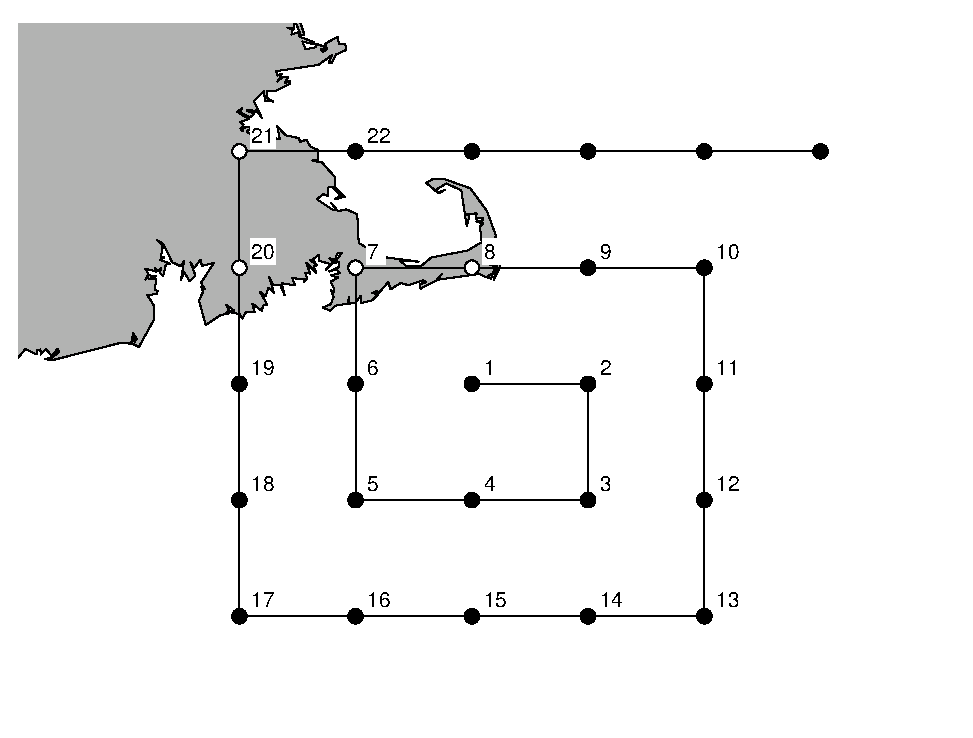
\epsfig{file=./num/wavetrack.eps,width=3.5in}
\caption{含陆地（阴影）的近岸规则计算网格上的追踪螺旋示例。黑点表示活动网格点，白点表示非活动（干）网格点。}
         \label{fig:wavetrack} \botline
\end{center}
\end{figure}

\begin{equation}
    GoF_{i} = {\left( \frac{T_\mathrm{p} - \tilde{T}^\mathrm{n}_{\mathrm{p},i}}{\Delta T_\mathrm{n}} \right)}^2 + 
                     {\left( \frac{\theta_\mathrm{p} - \tilde{\theta}^\mathrm{n}_{\mathrm{p},i}}{\Delta\theta_\mathrm{n}} \right)}^2 +
                     {\left( \frac{H_\mathrm{m0} - \tilde{H}^\mathrm{n}_{\mathrm{m0},i}}{\Delta H_\mathrm{n}} \right)}^2\ \ ,
\label{eq:grdgof}
\end{equation} 

\noindent
其中 $\Delta T_\mathrm{n}$、$\Delta\theta_\mathrm{n}$ 和 $\Delta
H_\mathrm{n}$ 是合并判据 \citep{art:WHD13}。若对于最接近匹配，式~(\ref{eq:grdgof}) 右端前两项中任一项超过 1，则认为差异过大，并将一个新的波系分配给该分区。这里，相邻点搜索范围设为 1，因此最多可找到四个此前已关联的相邻点（例如位置 15 会有此前处理过的相邻点 3、4、5 和 14）。在某些情况下，需要迭代合并。

下一步是在时间上对这些波系进行相关。当前时间层 $t$ 的每个系统 $i$ 与上一时间层 $(t-1)$ 的系统 $j$ 中最接近的匹配相关联。该过程中考虑波系的三个特征，即：(i) 系统内的空间平均峰值波周期 $\tilde{T}^\mathrm{s}_{\mathrm{p},t,i}$，其中
$\mathrm{s}$ 表示系统平均；(ii) 空间平均峰值波向
$\tilde{\theta}^\mathrm{s}_{\mathrm{p},t,i}$；以及 (iii) 两个系统在地理空间中重叠的网格点数 $\cap_{i,j}$。这些特征组合形成以下 GoF 函数：

\begin{equation}
    GoF_{i,j} = {\left( \frac{\tilde{T}^\mathrm{s}_{\mathrm{p},t,i} - \tilde{T}^\mathrm{s}_{\mathrm{p},t-1,j}}{\Delta T_\mathrm{s}} \right)}^2 + 
                       {\left( \frac{\tilde{\theta}^\mathrm{s}_{\mathrm{p},t,i} - \tilde{\theta}^\mathrm{s}_{\mathrm{p},t-1,j}}{\Delta\theta_\mathrm{s}} \right)}^2 +
                       {\left( \frac{N_{t-1,j} - \cap_{i,j}}{0.5N_{t-1,j}} \right)}^2\ \ ,
\label{eq:timegof}
\end{equation} 

\noindent
其中 $\Delta T_\mathrm{s}$ 和 $\Delta\theta_\mathrm{s}$ 是合并判据，$N$ 是一个系统中的网格点总数，见 \cite{art:WHD13}。为使追踪过程聚焦于波场中的高能区域，每个系统的空间平均周期和峰值方向值都按有效波高的平方加权。当前时间层 $t$ 的系统 $i$ 被分配给上一时间层 $(t-1)$ 中使式~(\ref{eq:timegof}) 最小的系统 $j$。若对于使式~(\ref{eq:timegof}) 最小的系统，式~(\ref{eq:timegof}) 右端三项中任一项超过 1，则分配一个新的系统编号。对最后一项而言，这意味着最小空间重叠要求，此处任意设为 50\%。该项主要影响盆地尺度区域，因为此类区域中的系统通常小于计算区域。为提高稳健性，识别出的系统细节会保存五个时间层，之后释放系统关联。

\vssub
\subsection{~嵌套} \label{sub:num_nest}
\conthead{\ws}{H. L. Tolman}

\noindent
传统上，波浪模式只考虑单向嵌套，即由低分辨率网格向高分辨率网格提供边界数据。\ws{} 一直提供这种方法，相关内容见 \para\ref{sub:one_way}。在模式 3.14 版中，引入了多网格波浪模式驱动程序，考虑网格之间的完整双向嵌套。该方法见 \para\ref{sub:two_way}。下文图示考虑规则网格，但所讨论的原则同样适用于曲线网格和三角形网格。


% -------------------------------------------------------------
\vssub
\subsubsection{~传统单向嵌套} \label{sub:one_way}
\vssub

\begin{figure}
\begin{center}

\setlength{\unitlength}{0.001in}

\begin{picture}(3000,1800)(0,-1550)

\put(0200,-1200){\vector(1,0){2100}}
\put(2400,-1250){\makebox(400,100){\small 空间}}
\put(0300,-1300){\vector(0,1){1300}}
\put(0100, 0100){\makebox(400,100)[c]{\small 时间}}

\multiput(0300,-1200)(0,300){4}{\circle {50}}
\multiput(0600,-1200)(0,300){4}{\circle {50}}
\multiput(0900,-1200)(0,300){4}{\circle {50}}
\multiput(1200,-1200)(0,300){4}{\circle*{50}}
\multiput(1500,-1200)(0,300){4}{\circle {50}}
\multiput(1800,-1200)(0,300){4}{\circle {50}}
\multiput(2100,-1200)(0,300){4}{\circle {50}}

\put(0300,-0150){\makebox(600,100)[c]{“陆地”}}
\put(0900,-0200){\vector(-1,0){575}}

\put(1500,-0150){\makebox(600,100)[c]{海洋}}
\put(1500,-0200){\vector(1,0){875}}
				       
\put(0900, 0050){\makebox(600,100)[c]{边界数据}}
\put(1100,-1200){\dashbox{50}(0200,1150){}}

\put(1050,-1550){\makebox(600,100)[c]{边界格式}}
\put(1200,-1400){\dashbox{25}(0300,1100){}}

\put(1550,-0750){\makebox(600,100)[l]{内部格式}}
\put(1500,-0800){\vector(1,0){875}}

\end{picture}
\end{center}

\caption{{\file ww3\_shel} 中使用的传统单向嵌套方法。空间和时间上的一维表示，符号表示网格点。} \label{fig:nest1}
\botline
\end{figure}


常规波浪模式程序 {\file ww3\_shel} 考虑单个波浪模式网格。该程序包含将边界条件从大尺度运行传递到小尺度运行的选项。每次运行可同时接受一个边界条件数据集，并生成最多 9 个边界条件数据集。为在水深和流场不兼容时保证波能守恒，边界数据由能量谱 $F(\sigma,\theta)$ 组成。数据文件包含生成运行中网格点处的谱，以及在所请求边界点处插值谱所需的信息。因此，如果小尺度运行的输入点位于大尺度运行的网格线上，传输文件的大小就最小。作为输入使用时，谱会在每个全局时间步长 $\Delta t_g$ 上以谱分量线性插值的方式在空间和时间上插值。

在波浪模式中包含边界数据的数值方法如图~\ref{fig:nest1} 所示。活动边界点在网格中被指定，用于将海点与陆点或其他停用网格点分隔开。在活动边界点和海点之间，应用局地边界格式（通常为一阶）。在模式内部海点中，则使用所选传播格式。

传统单向嵌套方法的实际使用方面在附录~\ref{app:nest} 中有更详细讨论。


% -------------------------------------------------------------
\vssub
\subsubsection{~双向嵌套} \label{sub:two_way}
\vssub

模式 3.14 版包含在程序 {\file ww3\_multi} 中使用多网格或镶嵌方法进行波浪建模的选项 \citep{tol:Vict06a,
  tol:MMAB07b, tol:OMOD08b}。在该程序中，可考虑任意数量、任意分辨率的网格，并在每个相关模式时间步长上在网格之间交换数据。网格被赋予等级编号，较低等级对应较低分辨率，相同等级对应相近分辨率（但不一定完全相同）。网格之间考虑三类数据传输：

\begin{itemize}
\item 从低等级网格向高等级网格传输数据。
\item 从高等级网格向低等级网格传输数据。
\item 在相同等级网格之间传输数据。
\end{itemize}

从低等级网格向高等级网格传输数据，是通过向高等级网格提供边界数据来完成的，方式与上一节和图~\ref{fig:nest1} 中所述的传统单向嵌套方法相同。

\begin{figure}
\begin{center}

\setlength{\unitlength}{0.001in}

\begin{picture}(3000,1900)(0,-1600)

\multiput(0300,-1400)(0,300){6}{\circle {50}}
\multiput(0600,-1400)(0,300){6}{\circle {50}}
\multiput(0900,-1400)(0,300){6}{\circle {50}}
\multiput(1200,-1400)(0,300){6}{\circle {50}}
\multiput(1500,-1400)(0,300){6}{\circle {50}}
\multiput(1800,-1400)(0,300){6}{\circle {50}}
\multiput(2100,-1400)(0,300){6}{\circle {50}}
\multiput(2400,-1400)(0,300){6}{\circle {50}}
\multiput(2700,-1400)(0,300){6}{\circle {50}}

\multiput(0450,-1550)(300,0){8}{\dashbox{50}(0000,1800){}}
\multiput(0150,-1250)(0,300){5}{\dashbox{50}(2700,0000){}}

\multiput(0400,-1450)(0,800){3}{\circle*{100}}
\multiput(1400,-1450)(0,800){3}{\circle*{100}}
\multiput(2400,-1450)(0,800){3}{\circle*{100}}

\put(895,-1055){\framebox(1010,810){}}
\put(900,-1050){\framebox(1000,800){}}
\put(905,-1045){\framebox(990,790){}}

\end{picture}
\end{center}

\caption{双向嵌套方法中协调低等级网格与高等级网格的概念示意。$\circ$ 和虚线分别表示高等级网格点和网格单元，$\bullet$ 和实线分别表示低等级网格及其中心网格单元。}
\label{fig:nest2}
\botline
\end{figure}


当该方法与从高等级到低等级的数据传输结合时，就建立了完整的双向嵌套方法。在 {\file ww3\_multi} 中，当高等级网格在时间上“追上”低等级网格之后，会将低等级网格中的数据与高等级网格中的数据相协调。考虑到低等级网格的分辨率按定义低于高等级网格的分辨率，从高等级网格中的能量 $E_{h,j}$ 估计低等级网格中的波能 $E_{l,i}$ 的一种自然方式为

\begin{equation}
E_{l,i} = \sum w_{i,j} E_{h,j} \:\:\: , \label{eq:nest_hg1}
\end{equation}

\noindent
其中 $i$ 和 $j$ 是两个网格中的网格计数器，$w_{i,j}$ 是平均权重。权重可按与波能守恒一致的方式定义为：高等级网格中覆盖低等级网格单元 $i$ 的网格单元 $j$ 的面积，并用低等级网格单元 $i$ 的面积归一化。图~\ref{fig:nest2} 对此作了说明。为避免循环协调，低等级网格中为高等级网格提供边界数据的网格点不以这种方式更新。

\input{zh/num/fig_nest3_zh}

相同等级的重叠网格不能使用上述双向嵌套技术来一致地交换数据。相反，所有这类网格都先传播一个时间步长，随后如图~\ref{fig:nest3} 所示对网格进行协调。对于网格 1（图~\ref{fig:nest3} 中的 $\circ$），可区分两个区域。在区域 C 中，自上次协调以来，边界影响已传播进入网格。实际穿透深度取决于数值格式的模板宽度以及传播时间步数。在区域 A 和 B 中，来自边界的信息尚未穿透，因此该区域可视为网格 1 的“内部”。类似地，区域 A 表示网格 2（图~\ref{fig:nest3} 中的 $\bullet$）的边界穿透深度，而 B 和 C 表示网格 2 的内部。网格 1 和网格 2 之间一种简单且一致的协调方法，是在区域 A 中仅使用网格 1 的数据（必要时将网格 1 的数据插值到网格 2 的网格点），并在区域 C 中仅使用网格 2 的数据。在区域 B 中，两个网格的内部部分重叠，可通过使用两个网格的加权平均获得一致解。注意，该方法很容易扩展到多个重叠网格。

注意，对于显式数值传播格式，以及具有相同分辨率且网格点重合的重叠网格，只要重叠区域足够宽，重叠网格的解就可以与兼容的单一网格解相同。

\vspace{\baselineskip} 
\noindent 
{\file ww3\_multi} 中的双向嵌套技术在很大程度上是自动化的。每个网格都独立准备，并具有自己首选的时间步进信息。每个网格期望从低等级网格获得边界数据的位置，会像单向嵌套方法一样标记。实现双向嵌套技术所需的所有其他簿记操作都是自动化的，不过可能需要若干次迭代，以确保每个网格中定义的所有输入边界点都能从多网格应用中的其他网格获得边界数据。作为替代，每个网格也可像传统嵌套方法一样从外部数据文件获取数据。在当前实现中，每个网格必须从单个文件或从多网格应用中的其他网格获得全部边界数据，但不能同时从文件和网格接收数据。关于为同时运行所有网格而开发的管理算法，详见 \citet[section 3.4]{tol:MMAB07b} 和 \cite{tol:OMOD08b}，此处不再重复。

注意，{\file ww3\_multi} 中使用的网格不需要具有相同的谱离散。谱会在 {\file
ww3\_multi} 中即时转换。该方法所用数值技术的细节可见 \citet[section 3.5.5]{tol:MMAB07b}。在这种方法中生成多网格可能很繁琐，并且需要保证网格之间的一致性以获得一致的模式结果。因此，\cite{tol:MMAB07a, tol:OMOD08a} 开发了自动网格生成工具。

